%!TEX root = ms.tex
\section*{Calculation of the rank percentile indicator}

In this section, we start by discussing the framework for calculating the rank percentile indicator. For publications, the indicator is based on the number of citations. We further propose utilizing an aggregation of rank percentile indicators for publications as the evaluation metric, based on which we then construct the indicator for scholars. We discuss the advantage of the proposed indicator compared to indicator based on existing evaluation metrics, such as the number of citations or h-index. 

\subsection*{Dataset}

The dataset from Google Scholar includes scholars in multiple disciplines from the top $10$ universities in the United States, which totals $14358$ scholars. It includes the citation history through $2016$ for each publication from these scholars; they contributed to more than $800,000$ publications total, which received approximately $100$ million citations collectively. The discipline for a scholar is determined by the area of interest specified on the Google Scholar page. For instance, a scholar and his/her publications are labeled as in the area of biology if the area of interest contains any of the following keywords: biology, genetic, neuroscience, or cell. An exploratory description of the dataset can be found in Supplemental Material (Figure S5 and Table S4). The dataset and the code to reproduce the results in this paper are available online at \url{https://github.com/sentian/SciImpactRanking}.

\subsection*{Framework for calculating the rank percentile indicator}
Recall that the four fundamental elements for the rank percentile indicator are as follows. 
\begin{itemize}
    \item Entity: publication (P) or scholar (S).
    \item Benchmark (b): the reference set to which the entity is compared.
    \item Metric (m): the measure that evaluates the performance of the entity.
    \item Age (t): the time when the evaluation is executed.
\end{itemize}
The rank percentile for publication $j$, P$_{m}^{jb}(t)$, is calculated in the following way.

\begin{enumerate}[label=(\arabic*)]
    \item Evaluate the publications in the benchmark by their performance at age $t$ (publications with life shorter than $t$ are not included). Utilize the evaluation metric to calculate the rank r$_{m}^{jb}(t)$ of publication $j$ against the publications in the benchmark. An average rank is assigned to r$_{m}^{jb}(t)$ if there exist other publications that have the same value of the metric. 
    \item The rank percentile is indicated by $\text{P}_{m}^{jb}(t)= \left(\text{r}_{m}^{jb}(t)-0.5\right)/N$.
\end{enumerate}
With the compromise $0.5/N$ in the final step, the median paper is assigned $50\%$ percentile, and the tails of the citation distribution are treated symmetrically~\cite{allen1914storage}. The above framework can be easily adapted to compute the rank percentile indicators for scholar $i$: S$_{m}^{ib}(t)$.


\subsection*{The rank percentile indicator for scholars}

For publication $j$, we utilize the number of citations by age $t$ as the evaluation metric and denote the rank percentile indicator as P$_c^{jb}(t)$. We further utilize the publication indicators to construct the rank percentile for scholars. For scholar $i$, the performance is determined by the qualities of the scholar's publications, in which each publication is evaluated via P$_c^{jb}(5)$, meaning the rank percentile for the publication at the fifth year since published. The evaluation metric for scholar $i$ is determined by aggregating the performance of all $N(t)$ papers that the scholar publishes by age $t$, that is $\displaystyle \sum_{j=1}^{N(t)} \text{P}_c^{jb}(5)$. We denote the resulting rank percentile indicator as S$_{P5}^{ib}(t)$, where P5 indicates the evaluation metric based on rank percentile indicator of publications at age $5$. In the discussion that follows, we utilize the simplified notations P$_c$ and S$_{P5}$ to refer to the publication and scholar rank percentiles in general, respectively. 

Figure \ref{fig:auti} presents an example of S$_{P5}$ for a random scholar in our dataset in which the benchmark includes all tenured professors in the top 10 universities, as ranked by the U.S. News. The scholar's career started in 2004, and our dataset tracks the citation information until 2016. The indicator S$_{P5}$ ranks the scholar to be in the top $40\%$ throughout the majority of their career. The figure indicates two other types of rank percentile indicators, S$_c$ and S$_h$, that utilize the number of citations and h-index score as evaluation metrics, respectively. We see that S$_h$ largely agrees with S$_{P5}$, and S$_c$ ranks the scholar lower than the other two indicators. 

% fig:auti
% an example of the scholar RP
\begin{figure}[ht!]
    \centering
    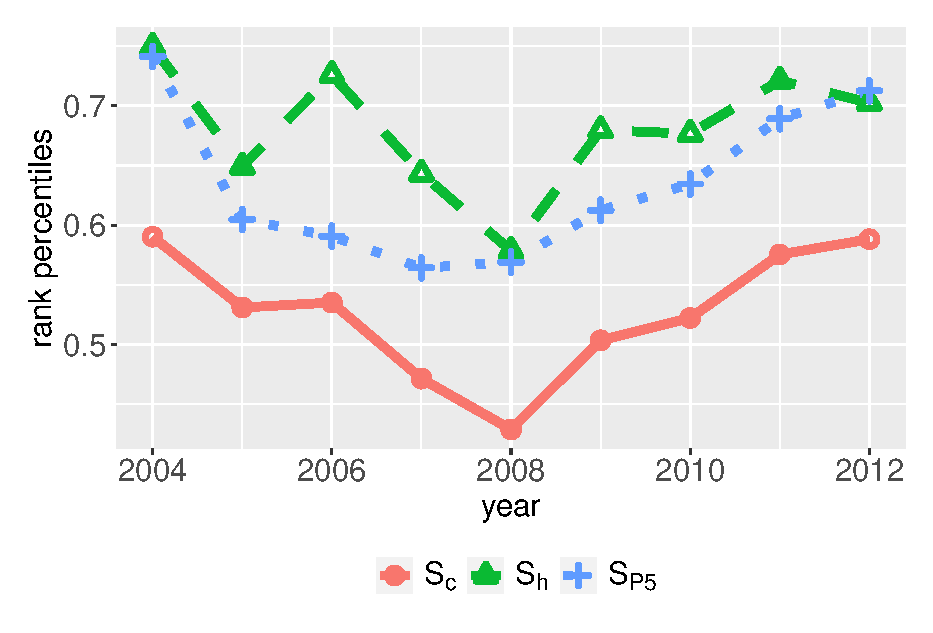
\includegraphics[width=0.6\textwidth]{figures/compare_autrp/auti.eps}
    \caption[rank percentile indicators for a random scholar]{The rank percentile indicators for a random scholar. The benchmark contains all tenured professors in the top-10 universities, as ranked by the U.S. News.}
    \label{fig:auti}
\end{figure}

The indicator S$_{P5}$ improves some major drawbacks of S$_c$ and S$_h$. First, it removes the seniority effect of publications. The evaluation metric for S$_c^{ib}(t)$ represents the citations that scholar $i$ receives by age $t$, which is the sum of citations for the scholar's publications by $t$. Compared to newly published works, publications with longer histories are more likely to attract citations and therefore contribute more to formulating S$_c$. A similar argument can be made for S$_h$. However, S$_{P5}$ treats the publications equally and evaluates them based on their performances at the publications' age of five. Additionally, a scholar who publishes a considerable number of low-impact works or participates in only a small number of high-impact projects can have a high value of S$_c$, since the absolute number of citations can be unlimited and is significantly influenced by extreme values. However, the S$_{P5}$ and S$_h$ of these scholars are not necessarily large, since these indicators limit the contribution of a single publication to be, at most, $1$ by definition of rank percentile and h-index score. Furthermore, compared to S$_h$, S$_{P5}$ penalizes scholars who are not truly innovative but carefully massage their h-index scores by publishing a number of papers that attract barely sufficient amounts of citations to increase their h-index scores. As long as a paper is among the top $h$ papers, the actual number of citations is irrelevant for h-index and S$_h$, but it can still impact S$_{P5}$. Finally, S$_{P5}$ requires less data compared to S$_c$ and S$_h$, since it only relies on the 5-year citation history of each publication. Hence, S$_{P5}$ is better suited to large-scale analysis.

We demonstrate the advantages of S$_{P5}$ by examining some extreme cases. We created three synthetic academic careers. Scholar A publishes a substantial number of publications throughout his/her career (more than $90\%$ of his/her cohorts in the benchmark), while all of the publications have little impact. Scholars B and C only publish one paper each at the beginning of their careers; B's paper is astonishing, while C's paper is average. Both scholars have an h-index equal to $1$ throughout their careers. Figure \ref{fig:simulated_authors} illustrates the rank percentile indicators for these three artificial scholars. We see that flooding low-impact publications can increase S$_c$ at the beginning of Scholar A's career. We also see that a single high-impact work improves the value S$_c$ throughout Scholar B's career; the author remains in the top $50\%$ at age $12$, as indicated by S$_c$. Both S$_{P5}$ and S$_h$ better characterize the performances of these authors. Finally, S$_h$ remains the same for Scholars B and C since they each have an h-index of $1$ throughout their careers. However, S$_{P5}$ considers that Scholar B's publication has a greater impact and therefore ranks higher than Scholar C. 

% fig:simulated_authors
% show the difference between various author rp
\begin{figure}[ht!]
    \centering
    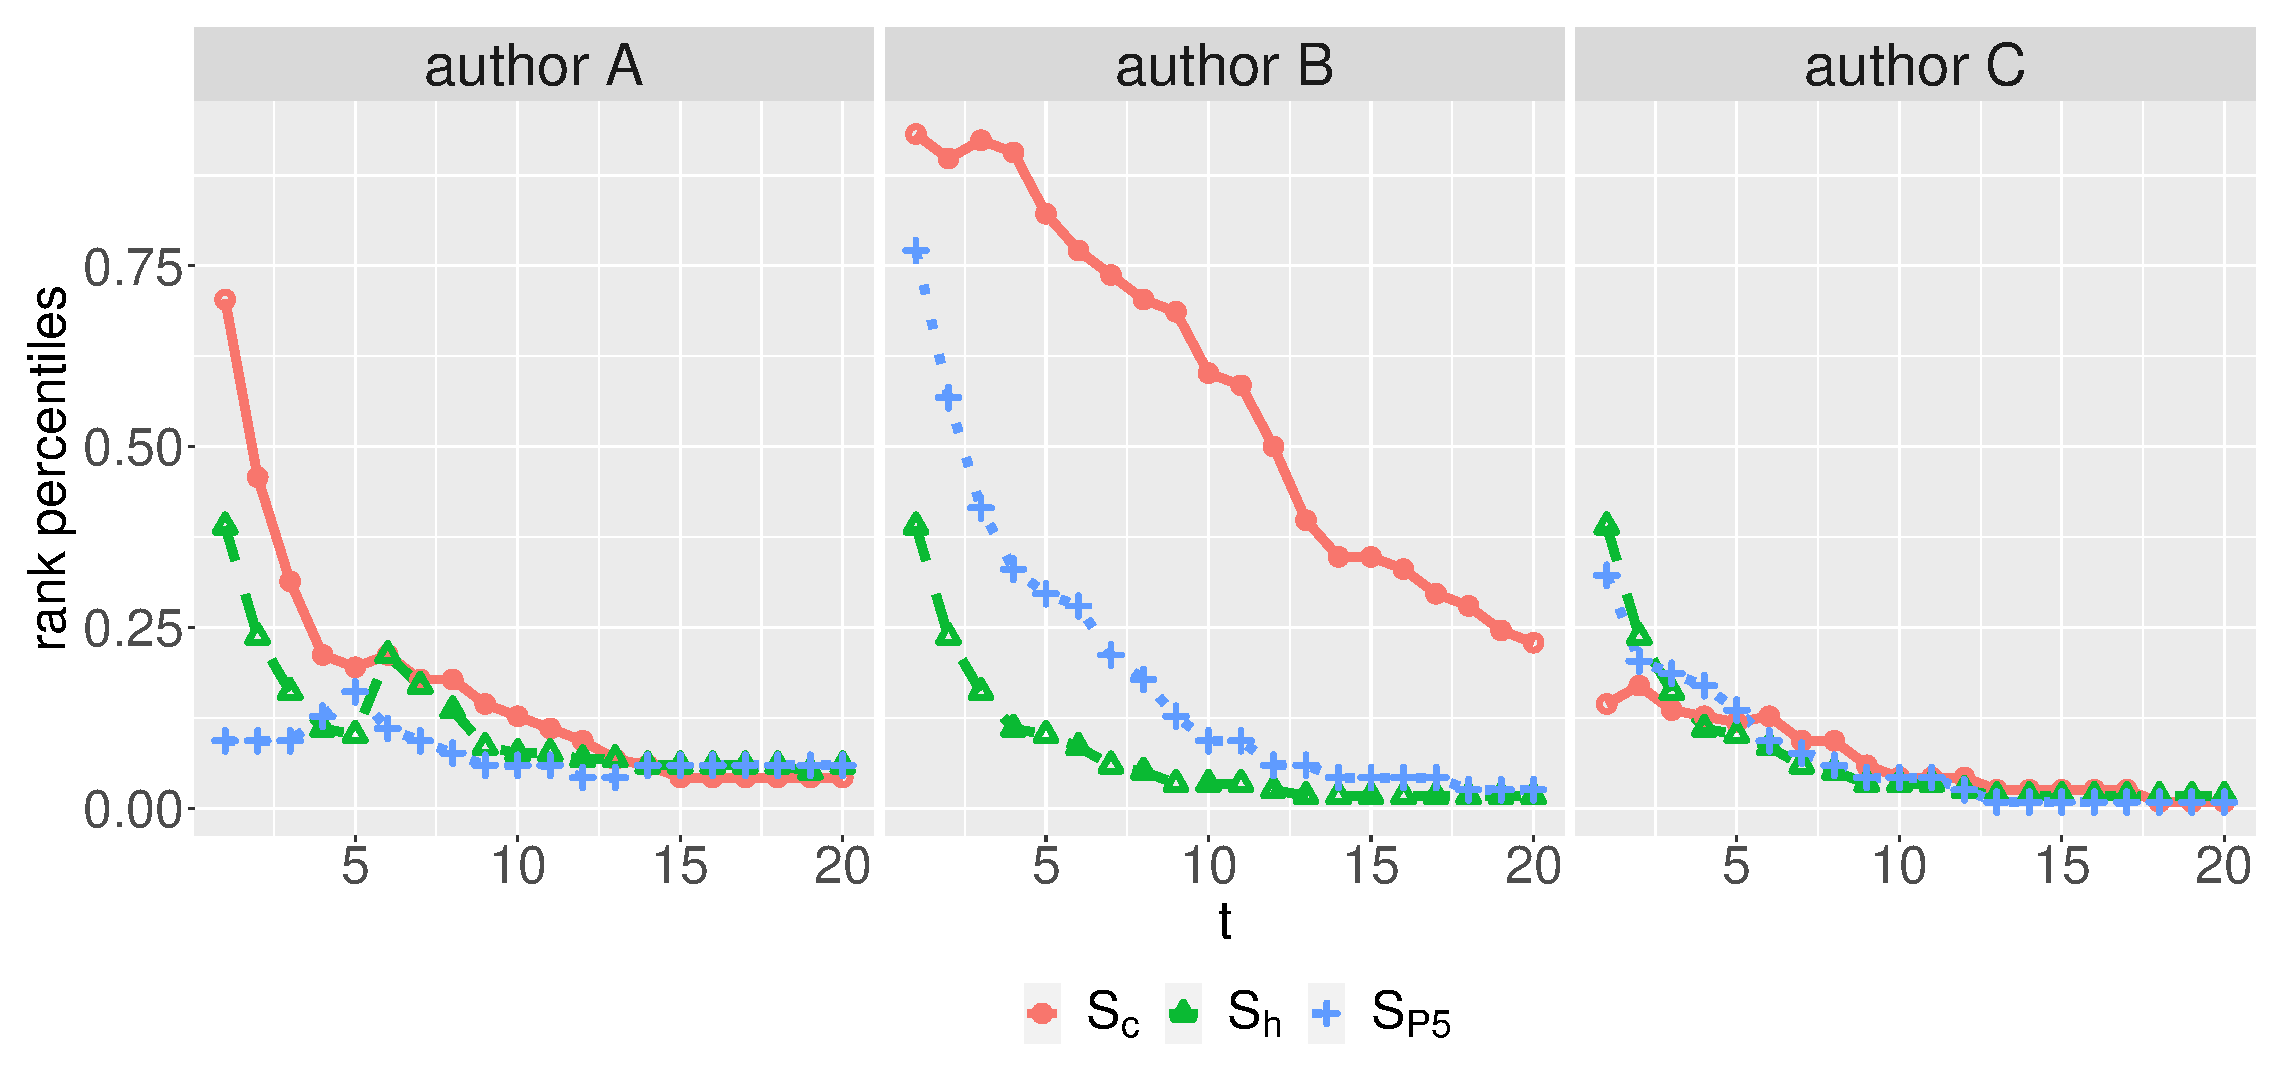
\includegraphics[width=\textwidth]{figures/compare_autrp/simulated_authors.eps}
    \caption[The advantage of S$_{it}^{P5}$ compared to other indicators]{Three artificial scholars illustrate the difference between various types of rank percentile indicators for scholars. Scholar A is highly productive at all ages, but all of the works have little impact. Scholars B and C only publish one paper each at age $1$; the paper of Scholar B has substantial impact, while the paper of Scholar C has medium impact. The h-index scores of Scholars B and C remain at $1$ throughout their careers. The benchmark includes scholars in biology who started their careers in $1990$.}
    \label{fig:simulated_authors}
\end{figure}

With the exception of the above-mentioned discrepancies, we present in Supplemental Material Section \ref{sec:suppl_similarity_autrp} that for the majority of scholars in our dataset, S$_{P5}$ largely agrees with S$_c$ and S$_h$. Furthermore, we consider utilizing various metrics to evaluate the publication, for example P$_c^{jb}(10)$ which is based on 10-year citation history. As we reveal Supplemental Material Section \ref{sec:suppl_robustness_P5}, the differences between the resultant rank percentile indicators and S$_{P5}$ are not statistically significant, thus indicating the robustness of S$_{P5}$. Intuitively, the publication percentile P$_c^{jb}(t)$ is highly stable over $t$, and therefore P$_c^{jb}(5)$ can be a reasonable indicator of the performance for the publication. The details will be discussed in the next section.

\section*{The predictability of rank percentile indicator}

In this section, we study the predictability of the rank percentile indicator. In general, we find the indicator to exhibit stability over time, and the indicator can be predicted via some simple linear regression models. 

\subsection*{The stationarity of the rank percentile indicator for scholars}

In the example of the tenure promotion, we utilized the rank percentile to compare the candidate with senior cohorts. The comparison is not valid if the candidate is more likely to attract citations than senior colleagues who started their careers years earlier. In such a case, it may well be the academic environment that results in a better performance of the candidate rather than the internal factors, such as creativity and productivity.

Figure \ref{fig:rp_stationarity} portrays S$_{P5}$ at age $10$, grouped by the starting year of academic careers. We see that S$_{P5}$ does not exhibit an obvious trend and is approximately stationary over the starting year of careers, thus providing empirical evidence for the validity of the rank percentile. 

\begin{figure}[ht!]
    \centering
    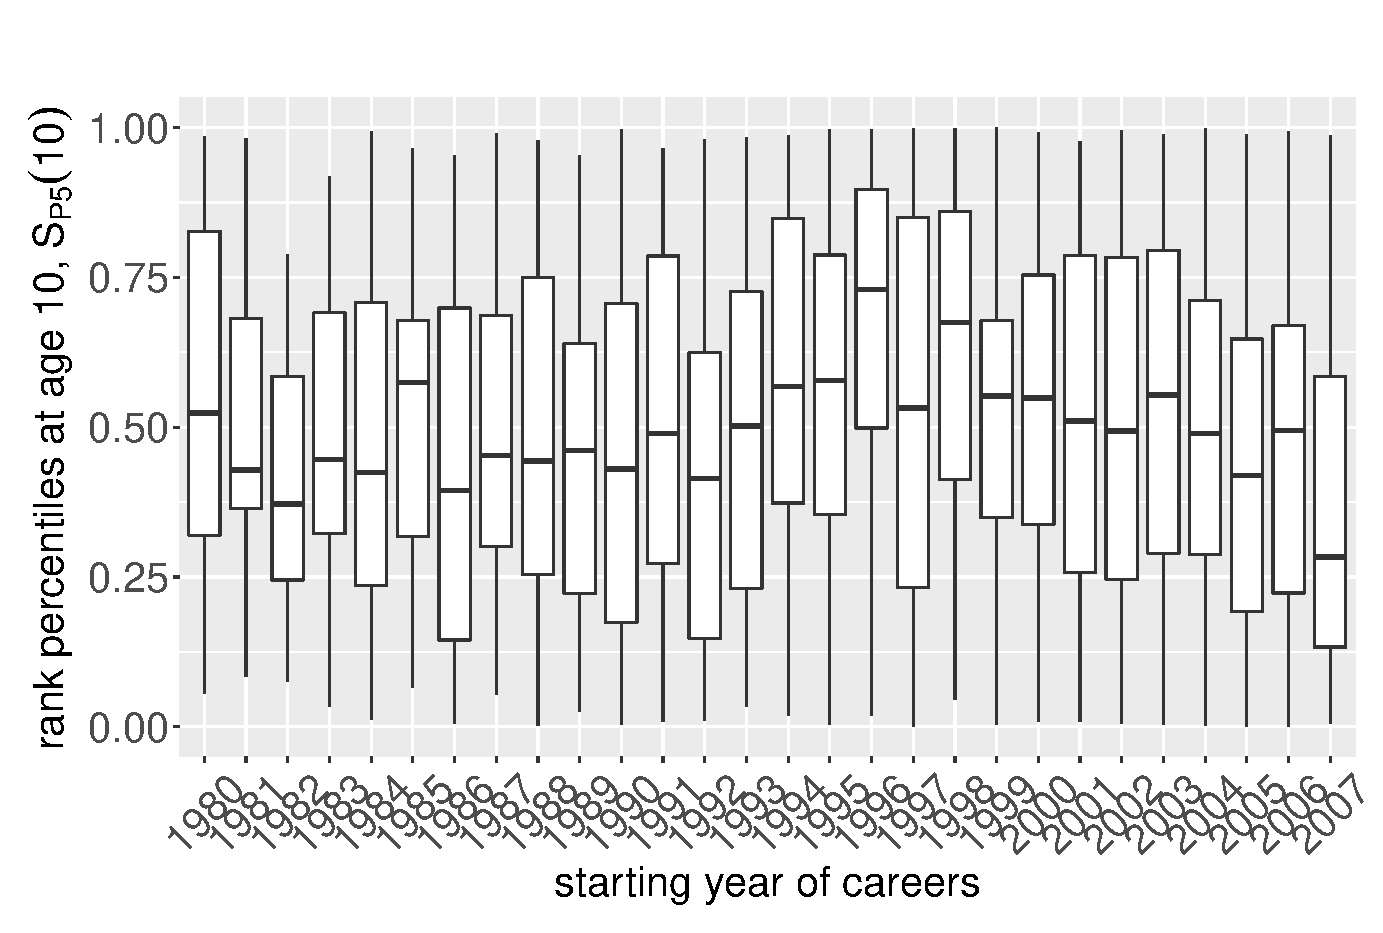
\includegraphics[width=0.6\textwidth]{figures/stationarity/rp_stationarity.eps}
    \caption[Stationarity of rank percentile indicators]{S$_{P5}(10)$ grouped by the starting years of academic careers. The benchmark contains all tenured professors in the top-10 universities, as ranked by the U.S. News.} 
    \label{fig:rp_stationarity}
\end{figure}

\subsection*{The predictability of rank percentile indicator}

Citations have been proven to lack long-term predictive power~\cite{Wang2013}. Figure \ref{fig:pred_cit_age} illustrates that papers with the same citations by the fifth year since published can have noticeably different citation paths and long-term effects. Additionally, exceptional and creative ideas typically require a lengthy period to be appreciated by the scientific community. As presented in Figure \ref{fig:pred_cit_cit}, the correlation between short- and long-term citations breaks down for the most highly-cited publications (the shaded rectangle). These problems can be largely avoided by utilizing rank percentile indicators, as evidenced in Figures \ref{fig:pred_rp_age} and \ref{fig:pred_rp_rp}. The considerable variation in the long-term effect of citations is restricted by utilizing rank percentiles. For publications with high impact, the correlation between short- and long-term effects persists when utilizing rank percentiles.

% publication rank percentile vs citations, predictability, Wang(2013)
\begin{figure}[ht!]
    \centering
    \begin{subfigure}[b]{0.48\textwidth}
     \centering
     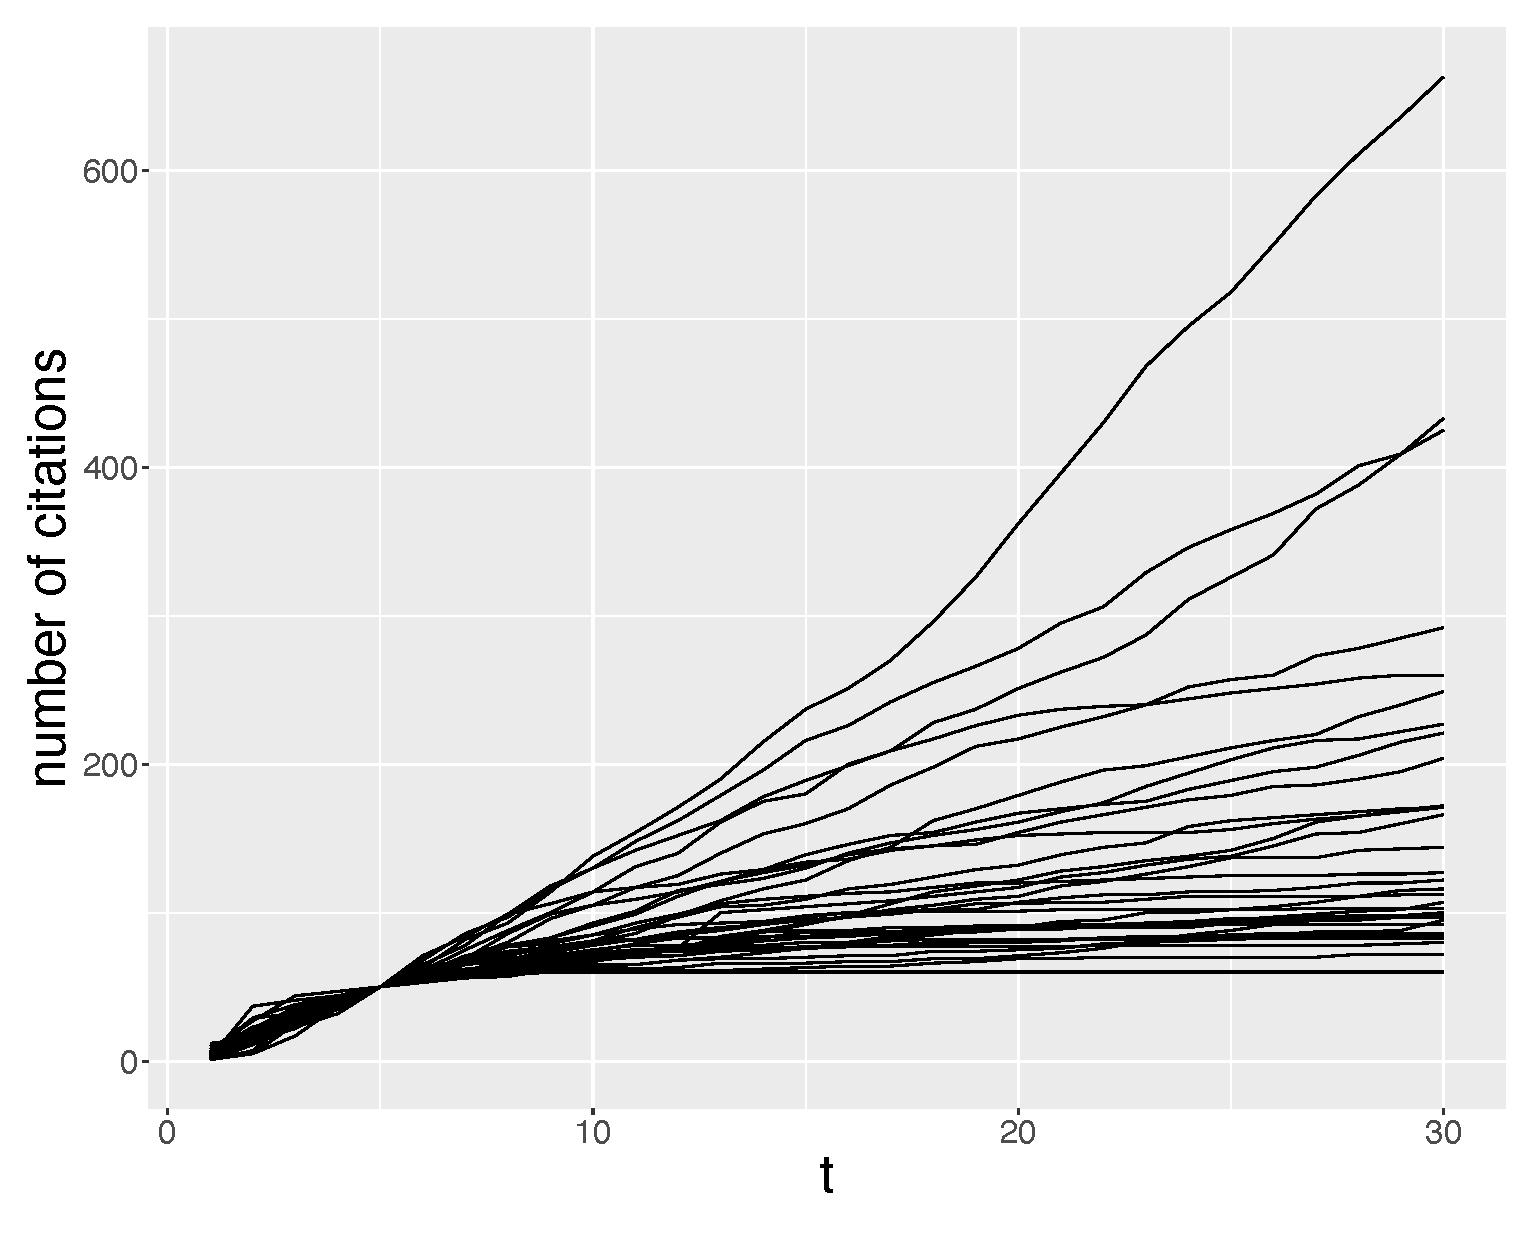
\includegraphics[width=\textwidth]{figures/pred_power/cit_t.eps}
     \caption{Number of citations versus age}
     \label{fig:pred_cit_age}
    \end{subfigure}
    \hfill
    \begin{subfigure}[b]{0.48\textwidth}
     \centering
     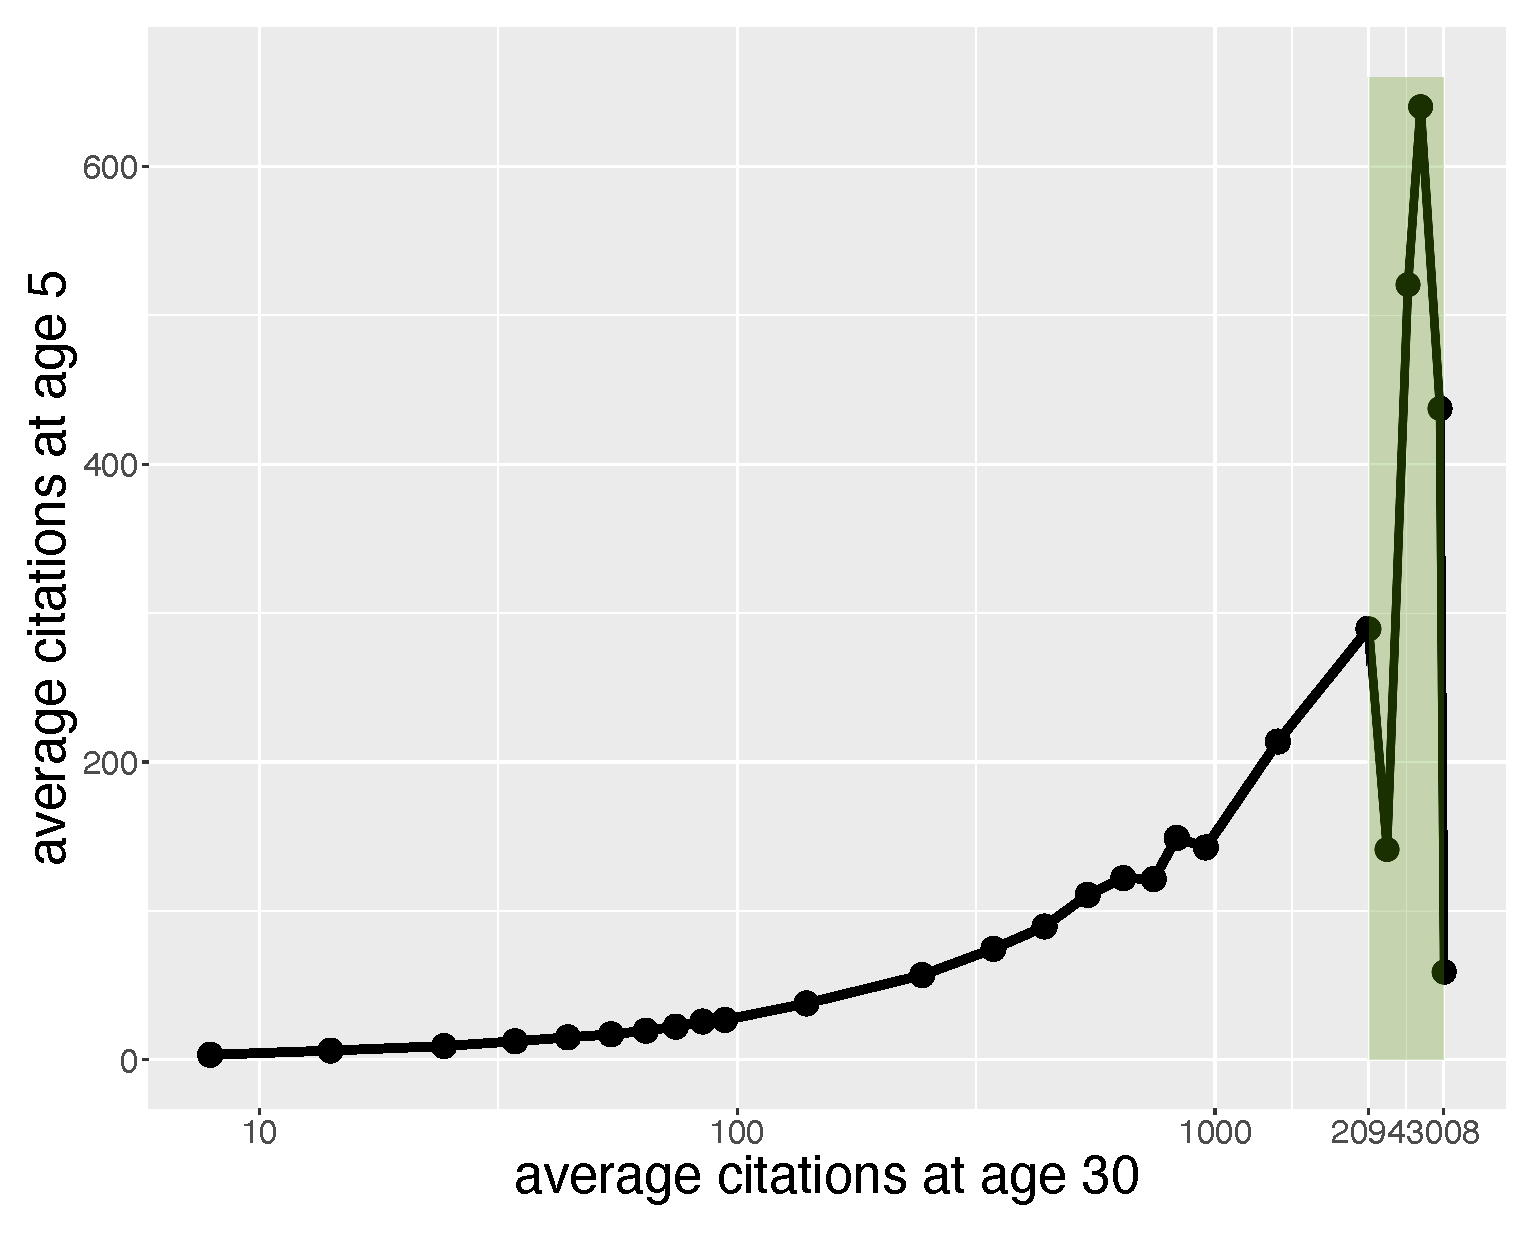
\includegraphics[width=\textwidth]{figures/pred_power/cit_cit.eps}
     \caption{Average citations at age $5$ versus those at age $30$}
     \label{fig:pred_cit_cit}
    \end{subfigure}
    \caption[Predictability of citations]{The predictability of citations. The benchmark contains the publications in biology. Figure \ref{fig:pred_cit_age} portrays the cumulative citations for publications that have $50$ citations by the fifth year since published. Figure \ref{fig:pred_cit_cit} displays the average citations by age $5$ versus the average citations by age $30$. The averages are calculated over groups of publications, which are prespecified by dividing the range of citations by age $30$ into equal intervals on the log scale. Note that we do not claim the originality of the figures, which have been illustrated via a different dataset~\cite{Wang2013}.}
    \label{fig:pub_cit_pred}
\end{figure}


\begin{figure}[ht!]
    \centering
    \begin{subfigure}[b]{0.495\textwidth}
     \centering
     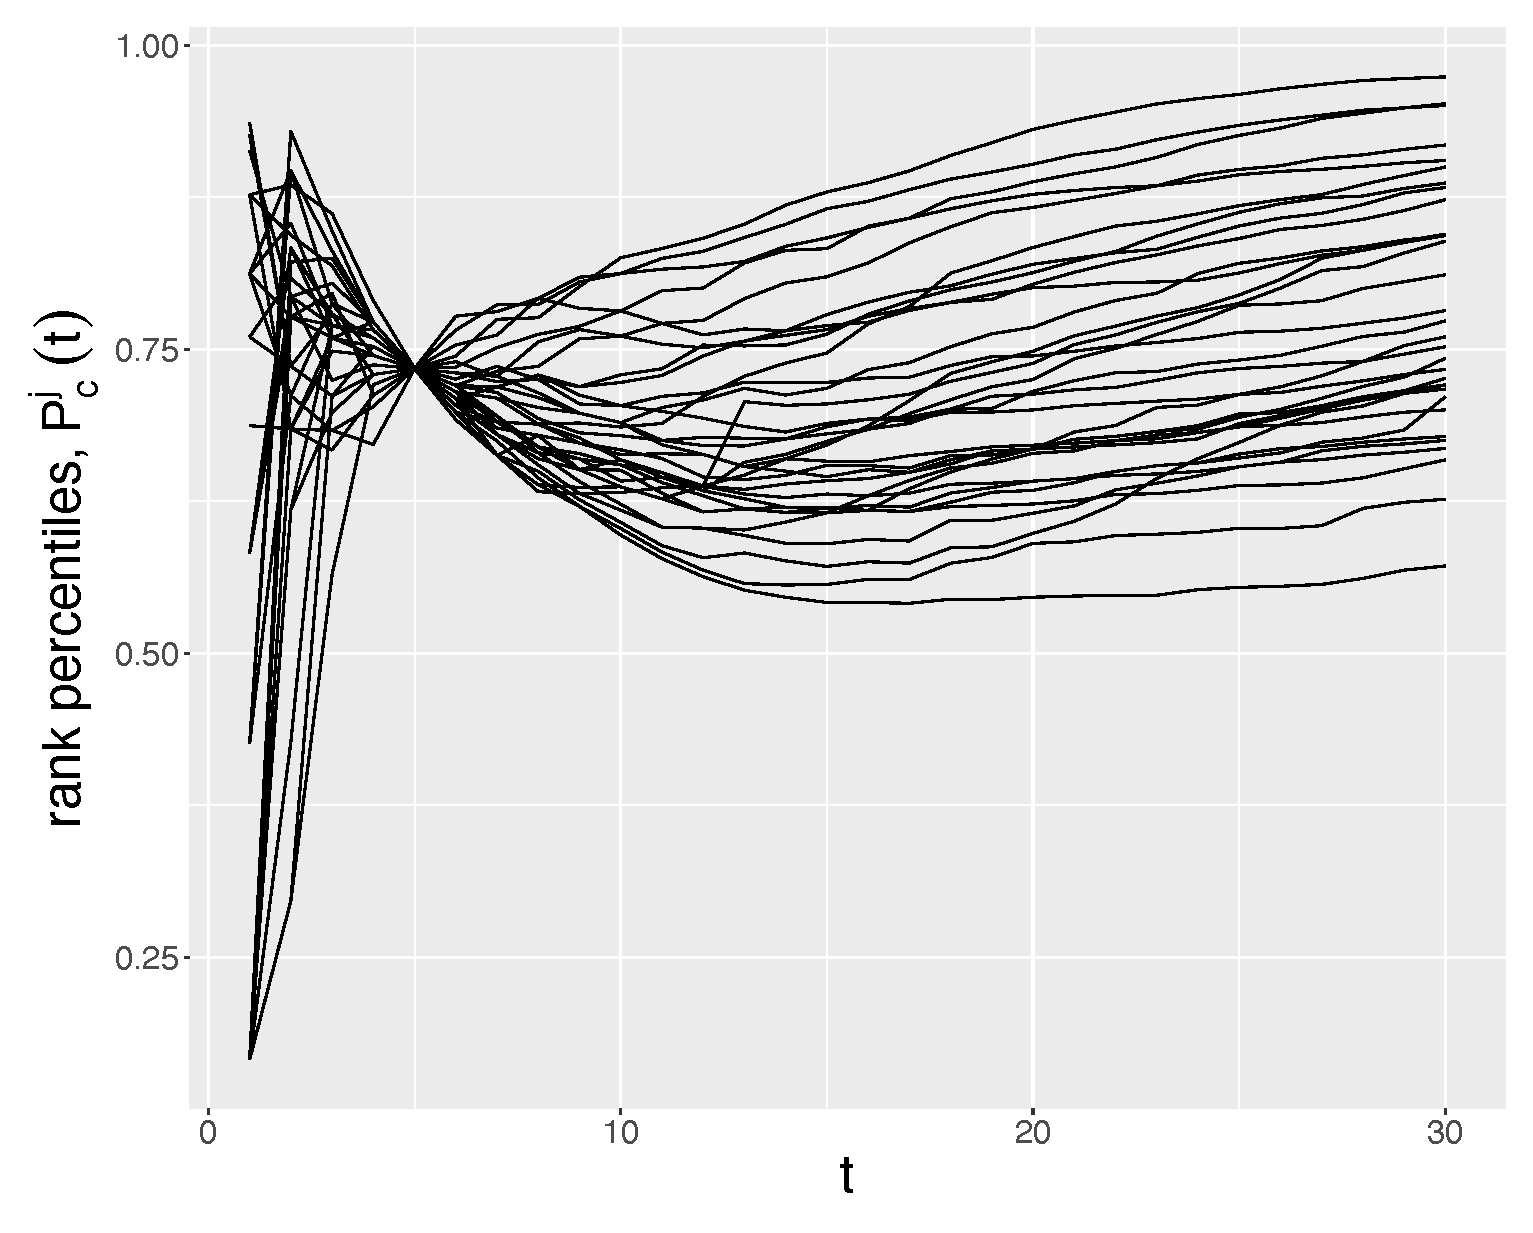
\includegraphics[width=\textwidth]{figures/pred_power/rp_t.eps}
     \caption{Rank percentiles P$_c$ versus age}
     \label{fig:pred_rp_age}
    \end{subfigure}
    \hfill
    \begin{subfigure}[b]{0.495\textwidth}
     \centering
     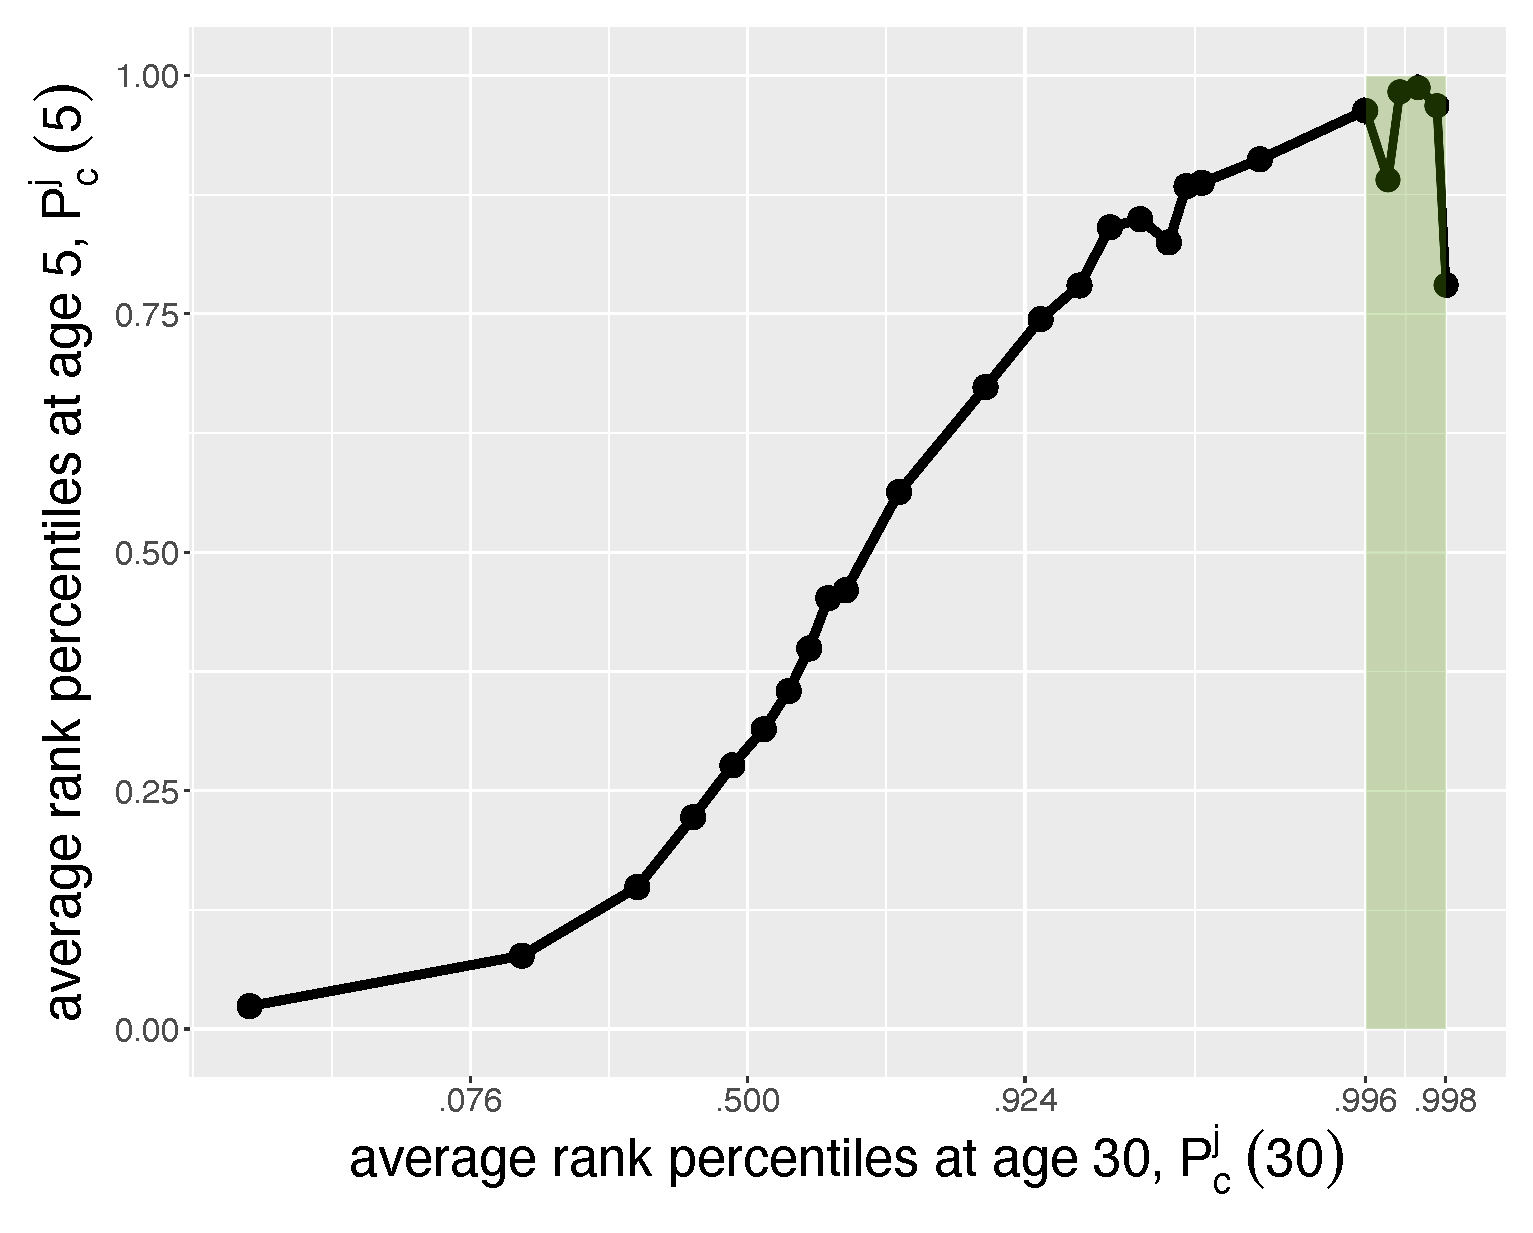
\includegraphics[width=\textwidth]{figures/pred_power/rp_rp.eps}
     \caption{Average P$_c$ at age $5$ versus those at age $30$}
     \label{fig:pred_rp_rp}
    \end{subfigure}
    \caption[Predictability of rank percentiles]{The predictability of rank percentiles. Figure \ref{fig:pred_rp_age} demonstrates the rank percentiles for the publications considered in Figure \ref{fig:pred_cit_age}. Figure \ref{fig:pred_rp_rp} presents the average of P$_c(5)$ versus the average of P$_c(30)$ for the same groups of publications as in Figure \ref{fig:pred_cit_cit}.}
    \label{fig:pub_rp_pred}
\end{figure}

We further characterize the predictability of rank percentile indicators. Figure \ref{fig:hm_rp_pub} presents the correlation between rank percentiles at two ages, P$_c^{jb}(t_1)$ and P$_c^{jb}(t_2)$ where $t_1<t_2$. We noticed overall large correlations for both benchmarks. The correlation diminishes as the forecast horizon $(t_2-t_1)$ increases, which simply reflects the difficulty of long-term forecasting. Additionally, the correlation increases as $t_1$ increases while holding the forecast horizon fix. This indicates that the performance of a senior publication is easier to predict, since the longer history removes more uncertainties regarding its performance. We further noticed a slightly higher predictive power when we restricted the benchmark to be the area of biology. 

Figure \ref{fig:hm_rp_aut} illustrates that the patterns discussed above generally hold for rank percentiles of scholars. The magnitude of correlations is smaller than those for publications, especially for long-term forecasts. This results from the fact that forecasting the future impact of future works is considerably more difficult than forecasting the future impact of existing works. Intuitively, predicting S$_{P5}^{ib}(t_2)$ involves predicting the performance of papers published before $t_1$ and predicting the performance of those published between $t_1$ and $t_2$. The former is predicting the future impact of existing works, while the latter is predicting the future impact of future works. However, predicting the publication indicator P$_c^{jb}(t_2)$ only involves predicting the future impact of publication $j$, which is a considerably easier task. Furthermore, when the forecast horizon increases while fixing $t_1$, additional future works are involved in predicting S$_{P5}^{ib}(t_2)$; therefore, we see that the correlation decreases more quickly than when we predict P$_c^{jb}(t_2)$. 

% publication rank percentile, heat map of correlations
\begin{figure}[ht!]
    \centering
    \begin{subfigure}[b]{0.8\textwidth}
        \centering
             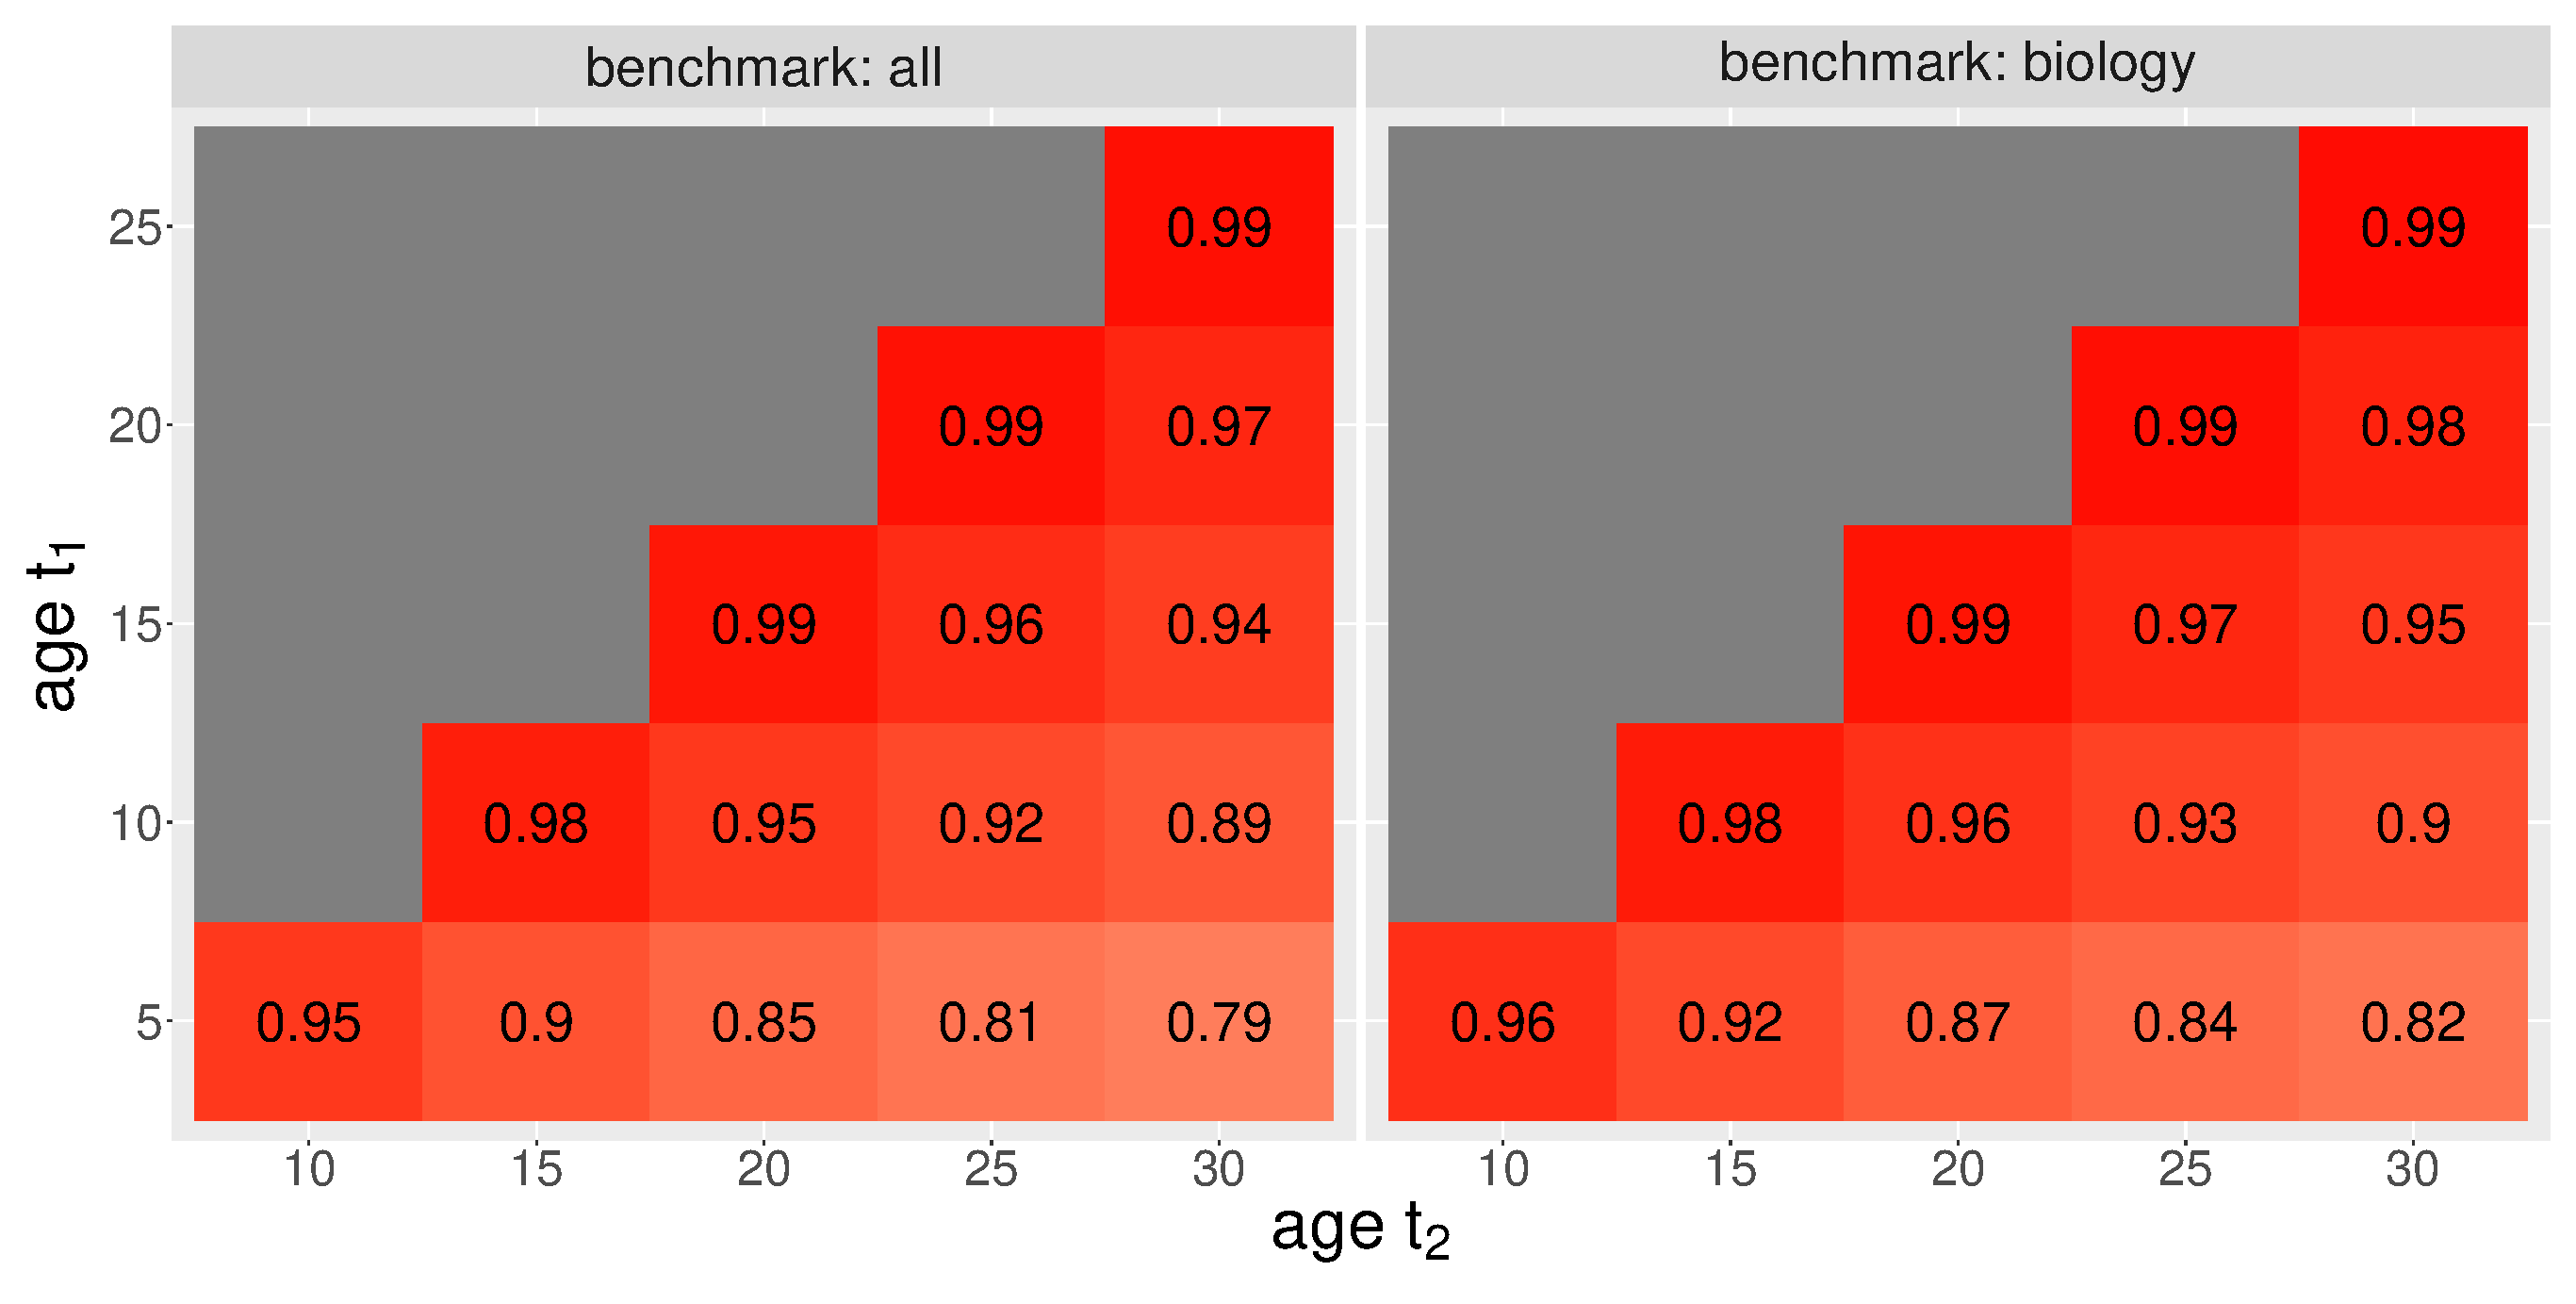
\includegraphics[width=\textwidth]{figures/pred_power/heatmap_cor_pub.eps}
         \caption{Correlation between P$_c^{jb}(t_1)$ and P$_c^{jb}(t_2)$}
         \label{fig:hm_rp_pub}
    \end{subfigure}

    \begin{subfigure}[b]{0.8\textwidth}
        \centering
             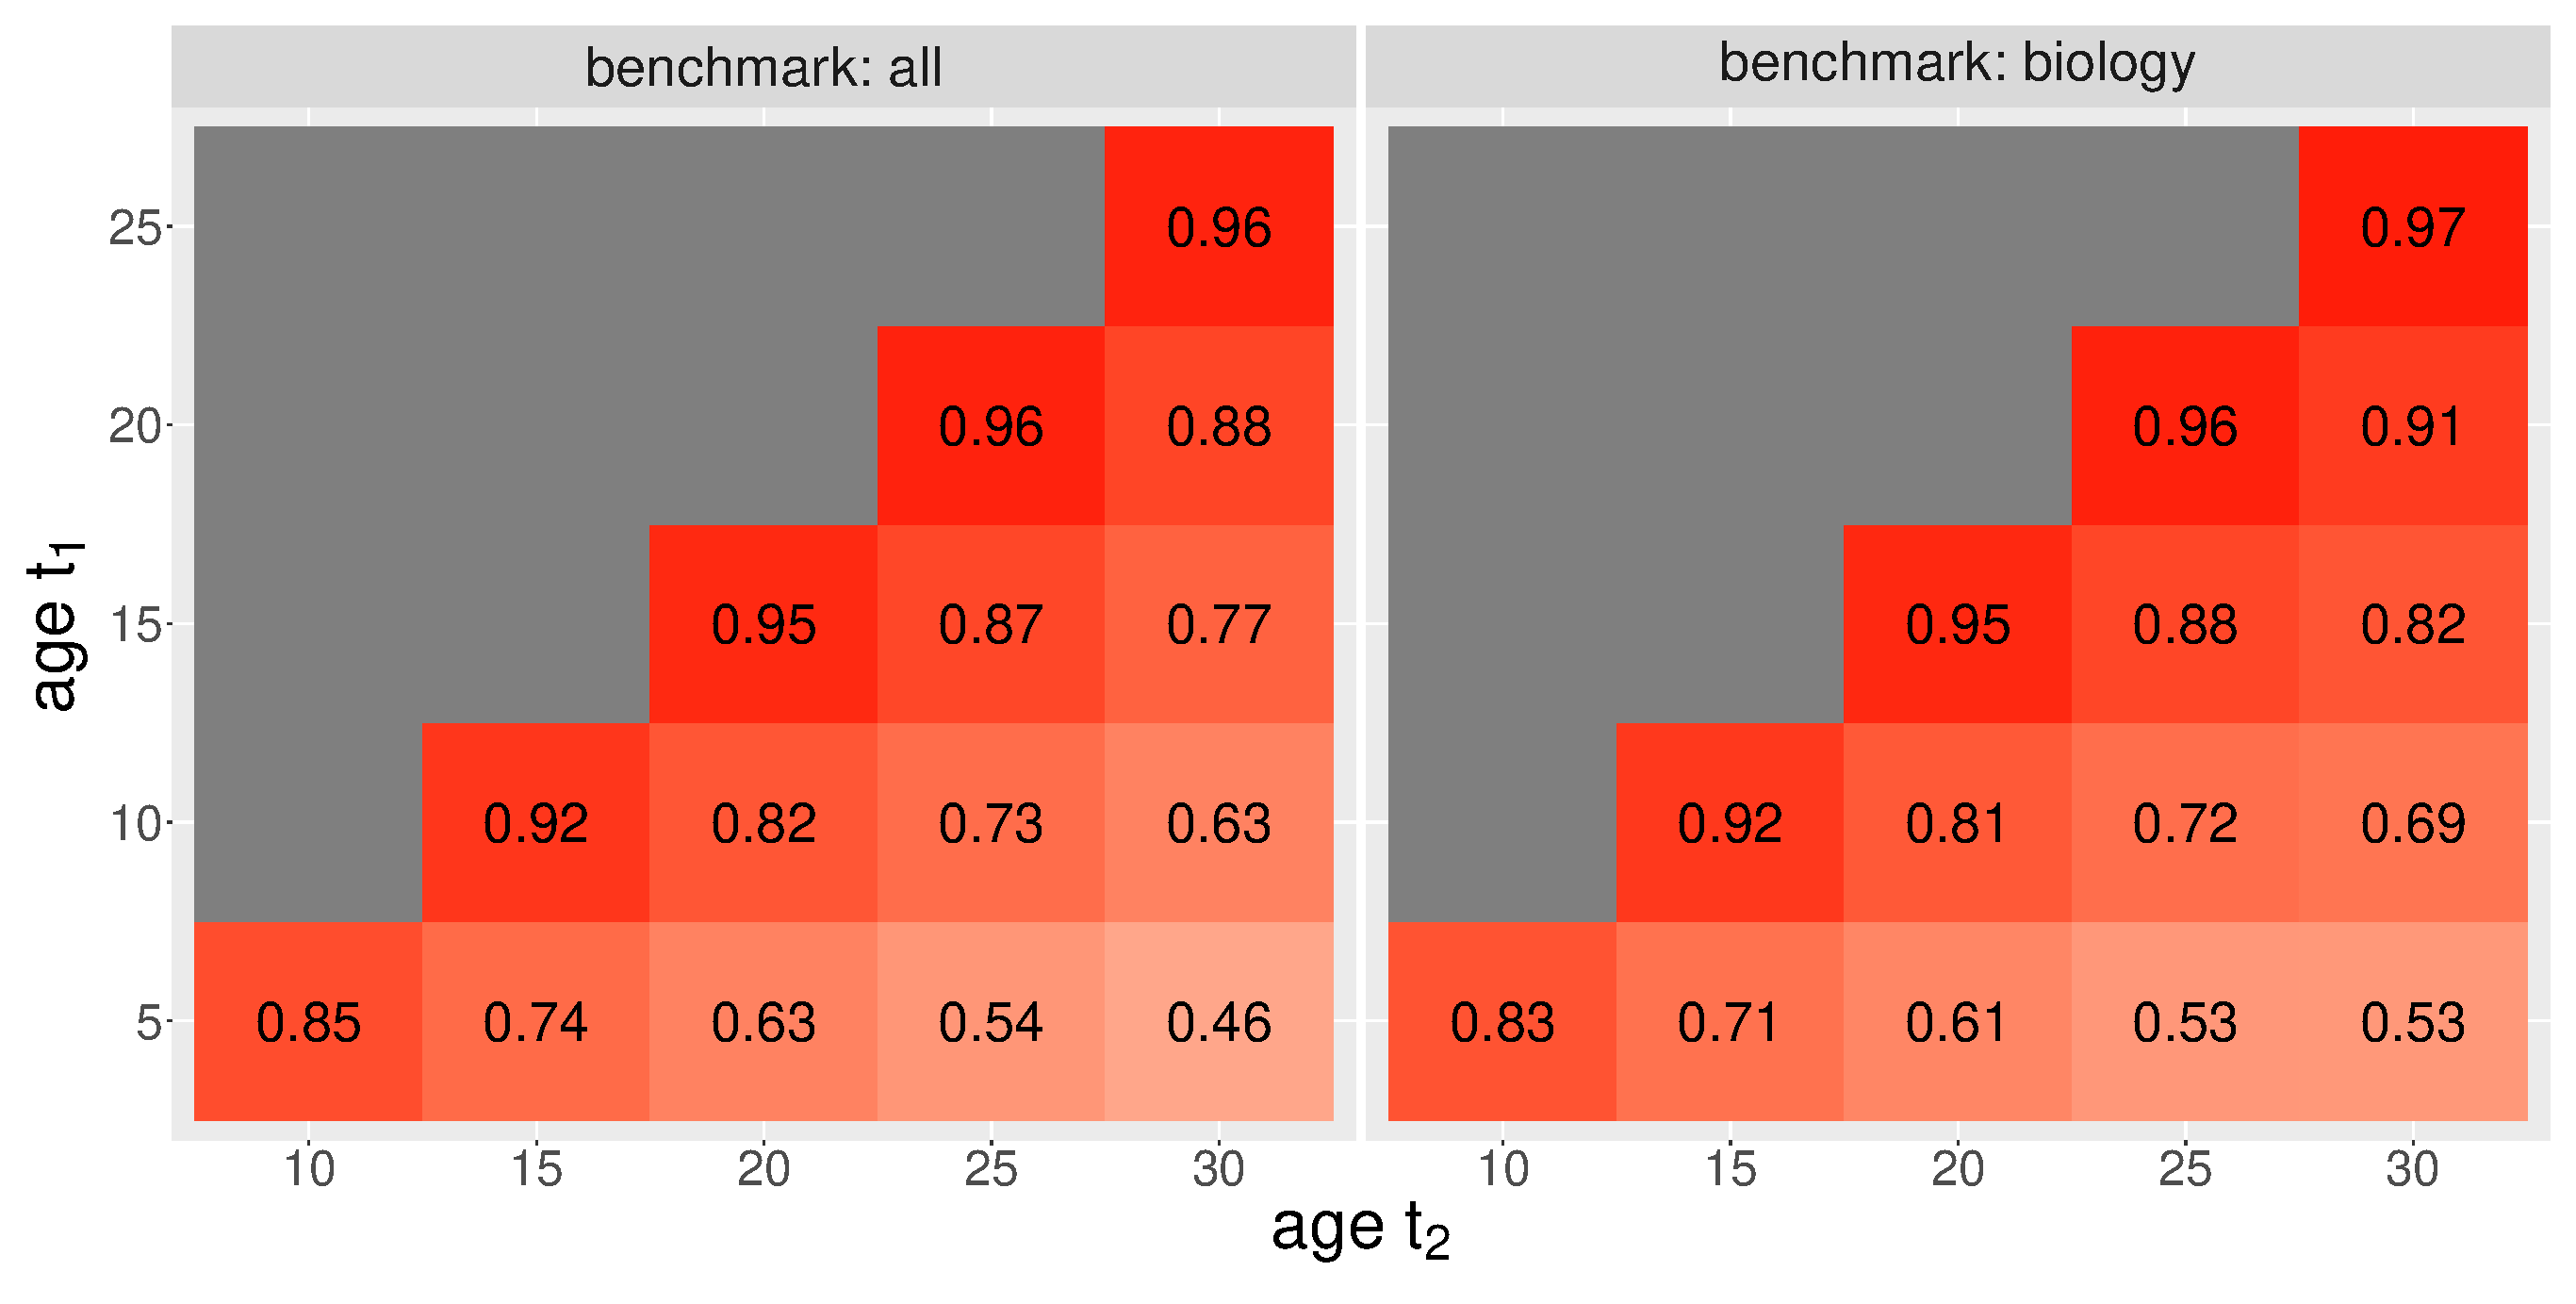
\includegraphics[width=\textwidth]{figures/pred_power/heatmap_cor_aut.eps}
         \caption{Correlation between S$_{P5}^{ib}(t_1)$ and S$_{P5}^{ib}(t_2)$}
         \label{fig:hm_rp_aut}
    \end{subfigure}

    \begin{subfigure}[b]{0.8\textwidth}
        \centering
             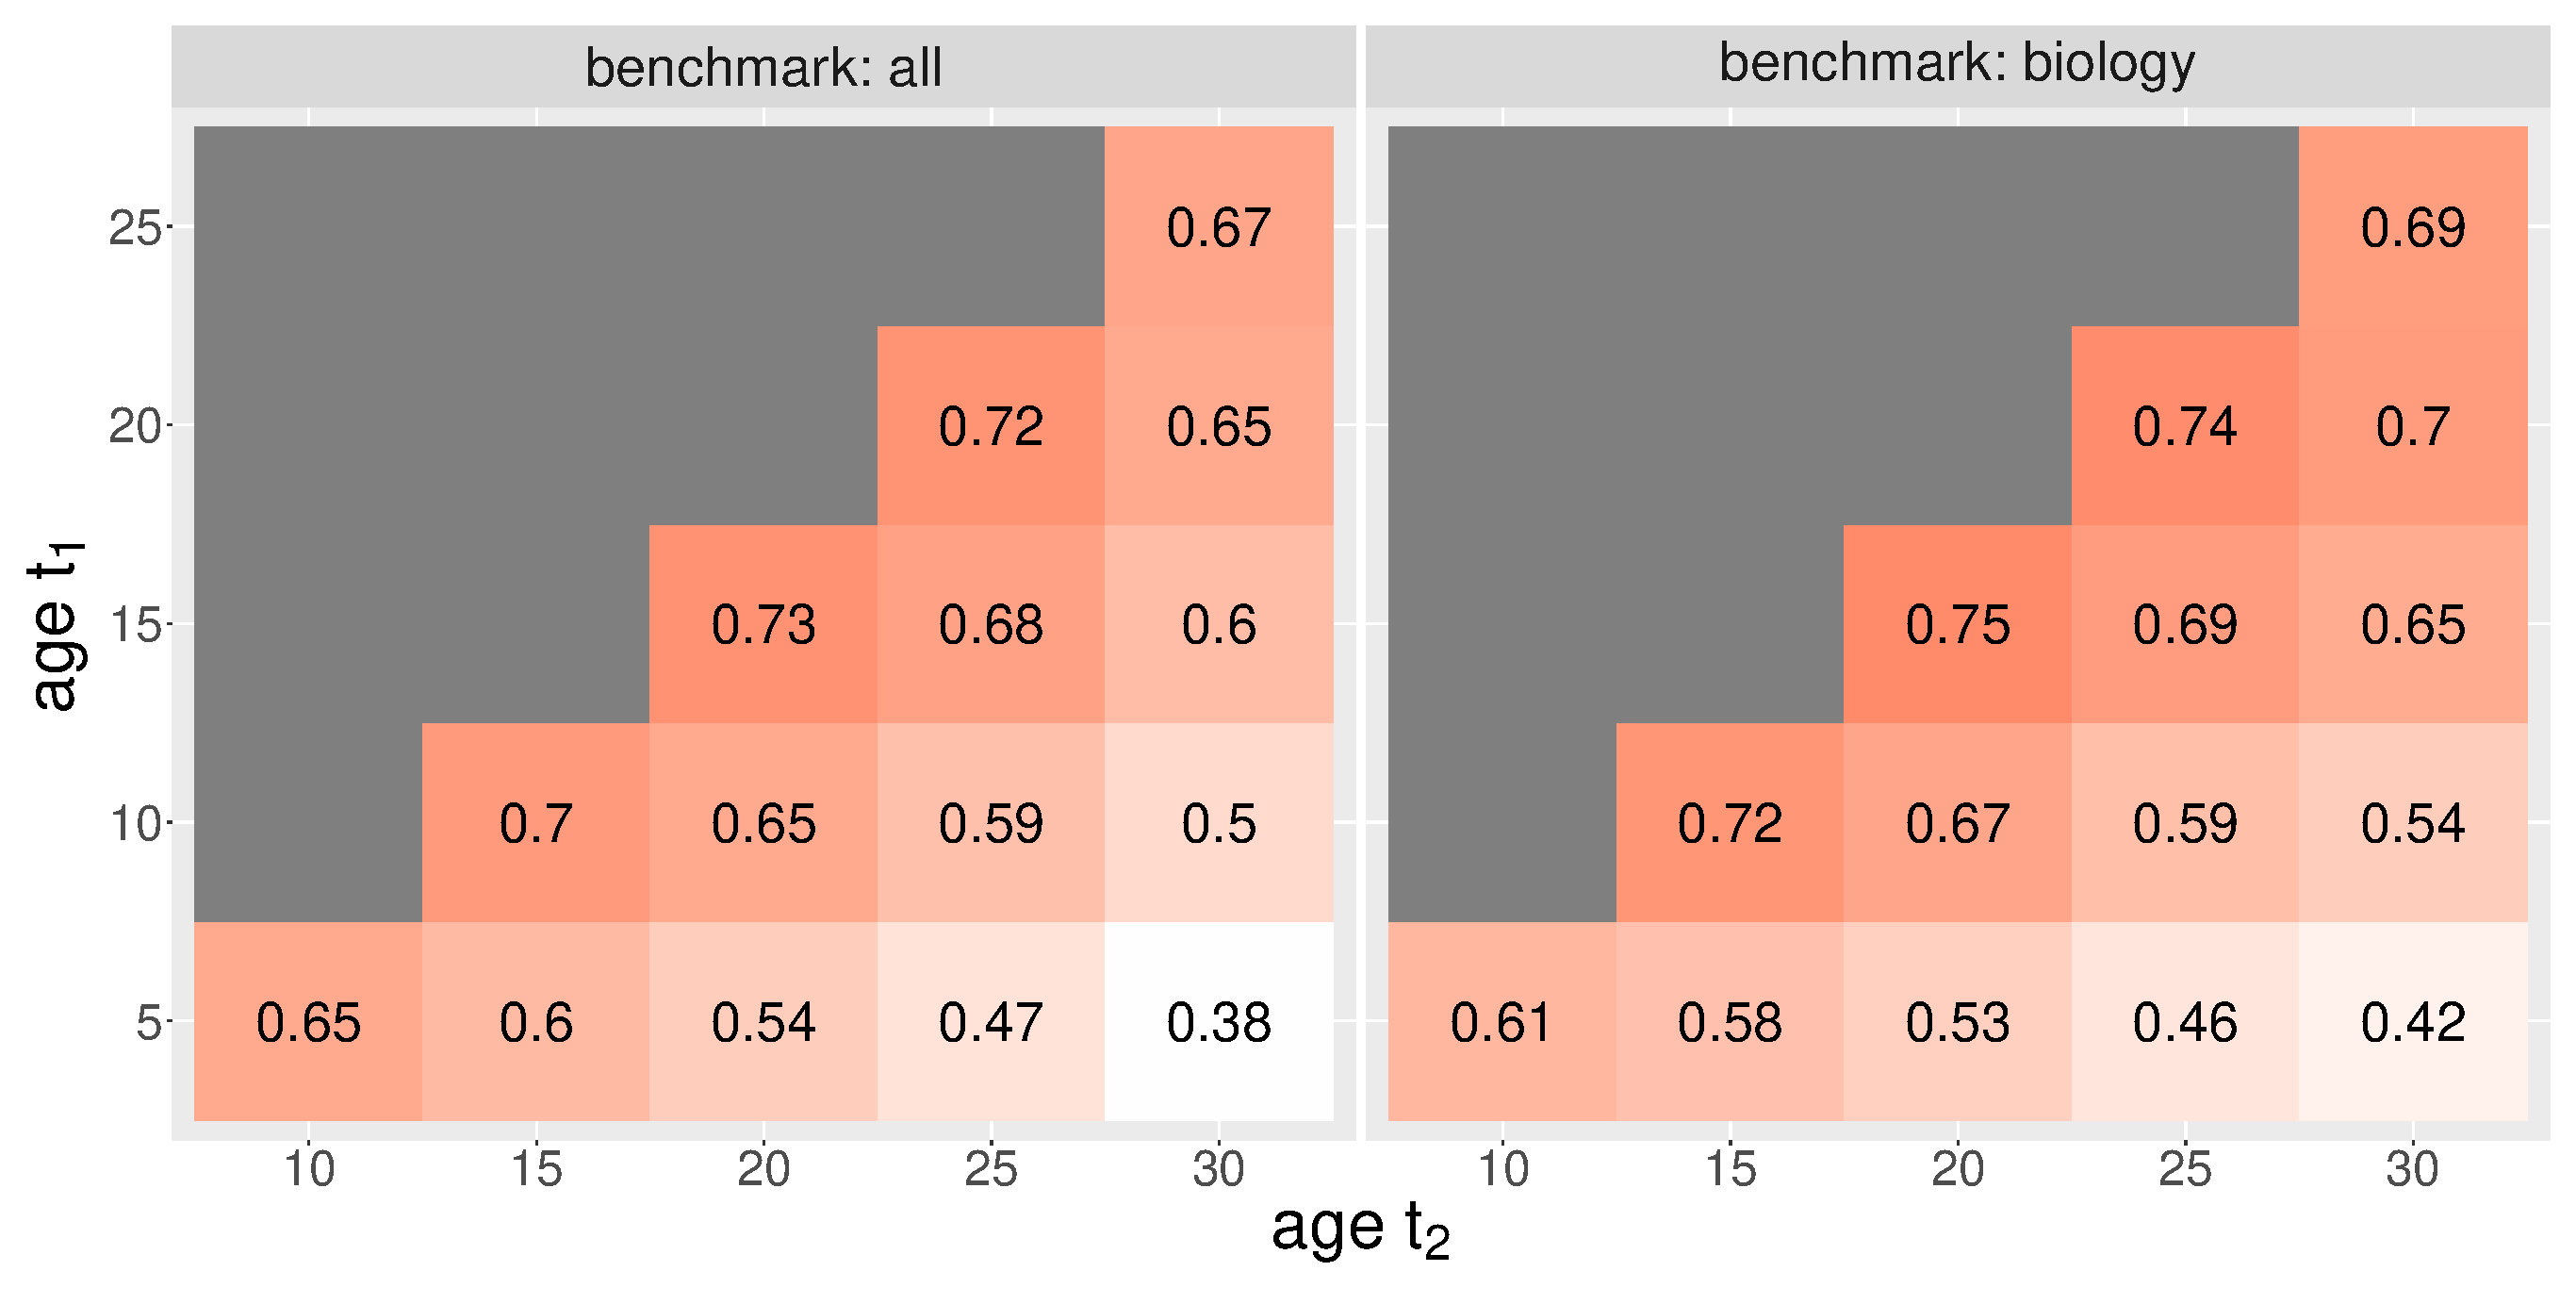
\includegraphics[width=\textwidth]{figures/pred_power/heatmap_cor_aut_future.eps}
         \caption{Correlation between S$_{P5}^{ib}(t_1)$ and S$_{P5}^{ib}(t_2 | t_1)$}
         \label{fig:hm_rp_aut_future}
    \end{subfigure}
    \caption[Correlations between rank percentiles at different ages]{The Pearson's correlation between rank percentile indicators at two different ages. }
    \label{fig:hm_rp}
\end{figure}

\begin{figure}[ht!]
    \centering
    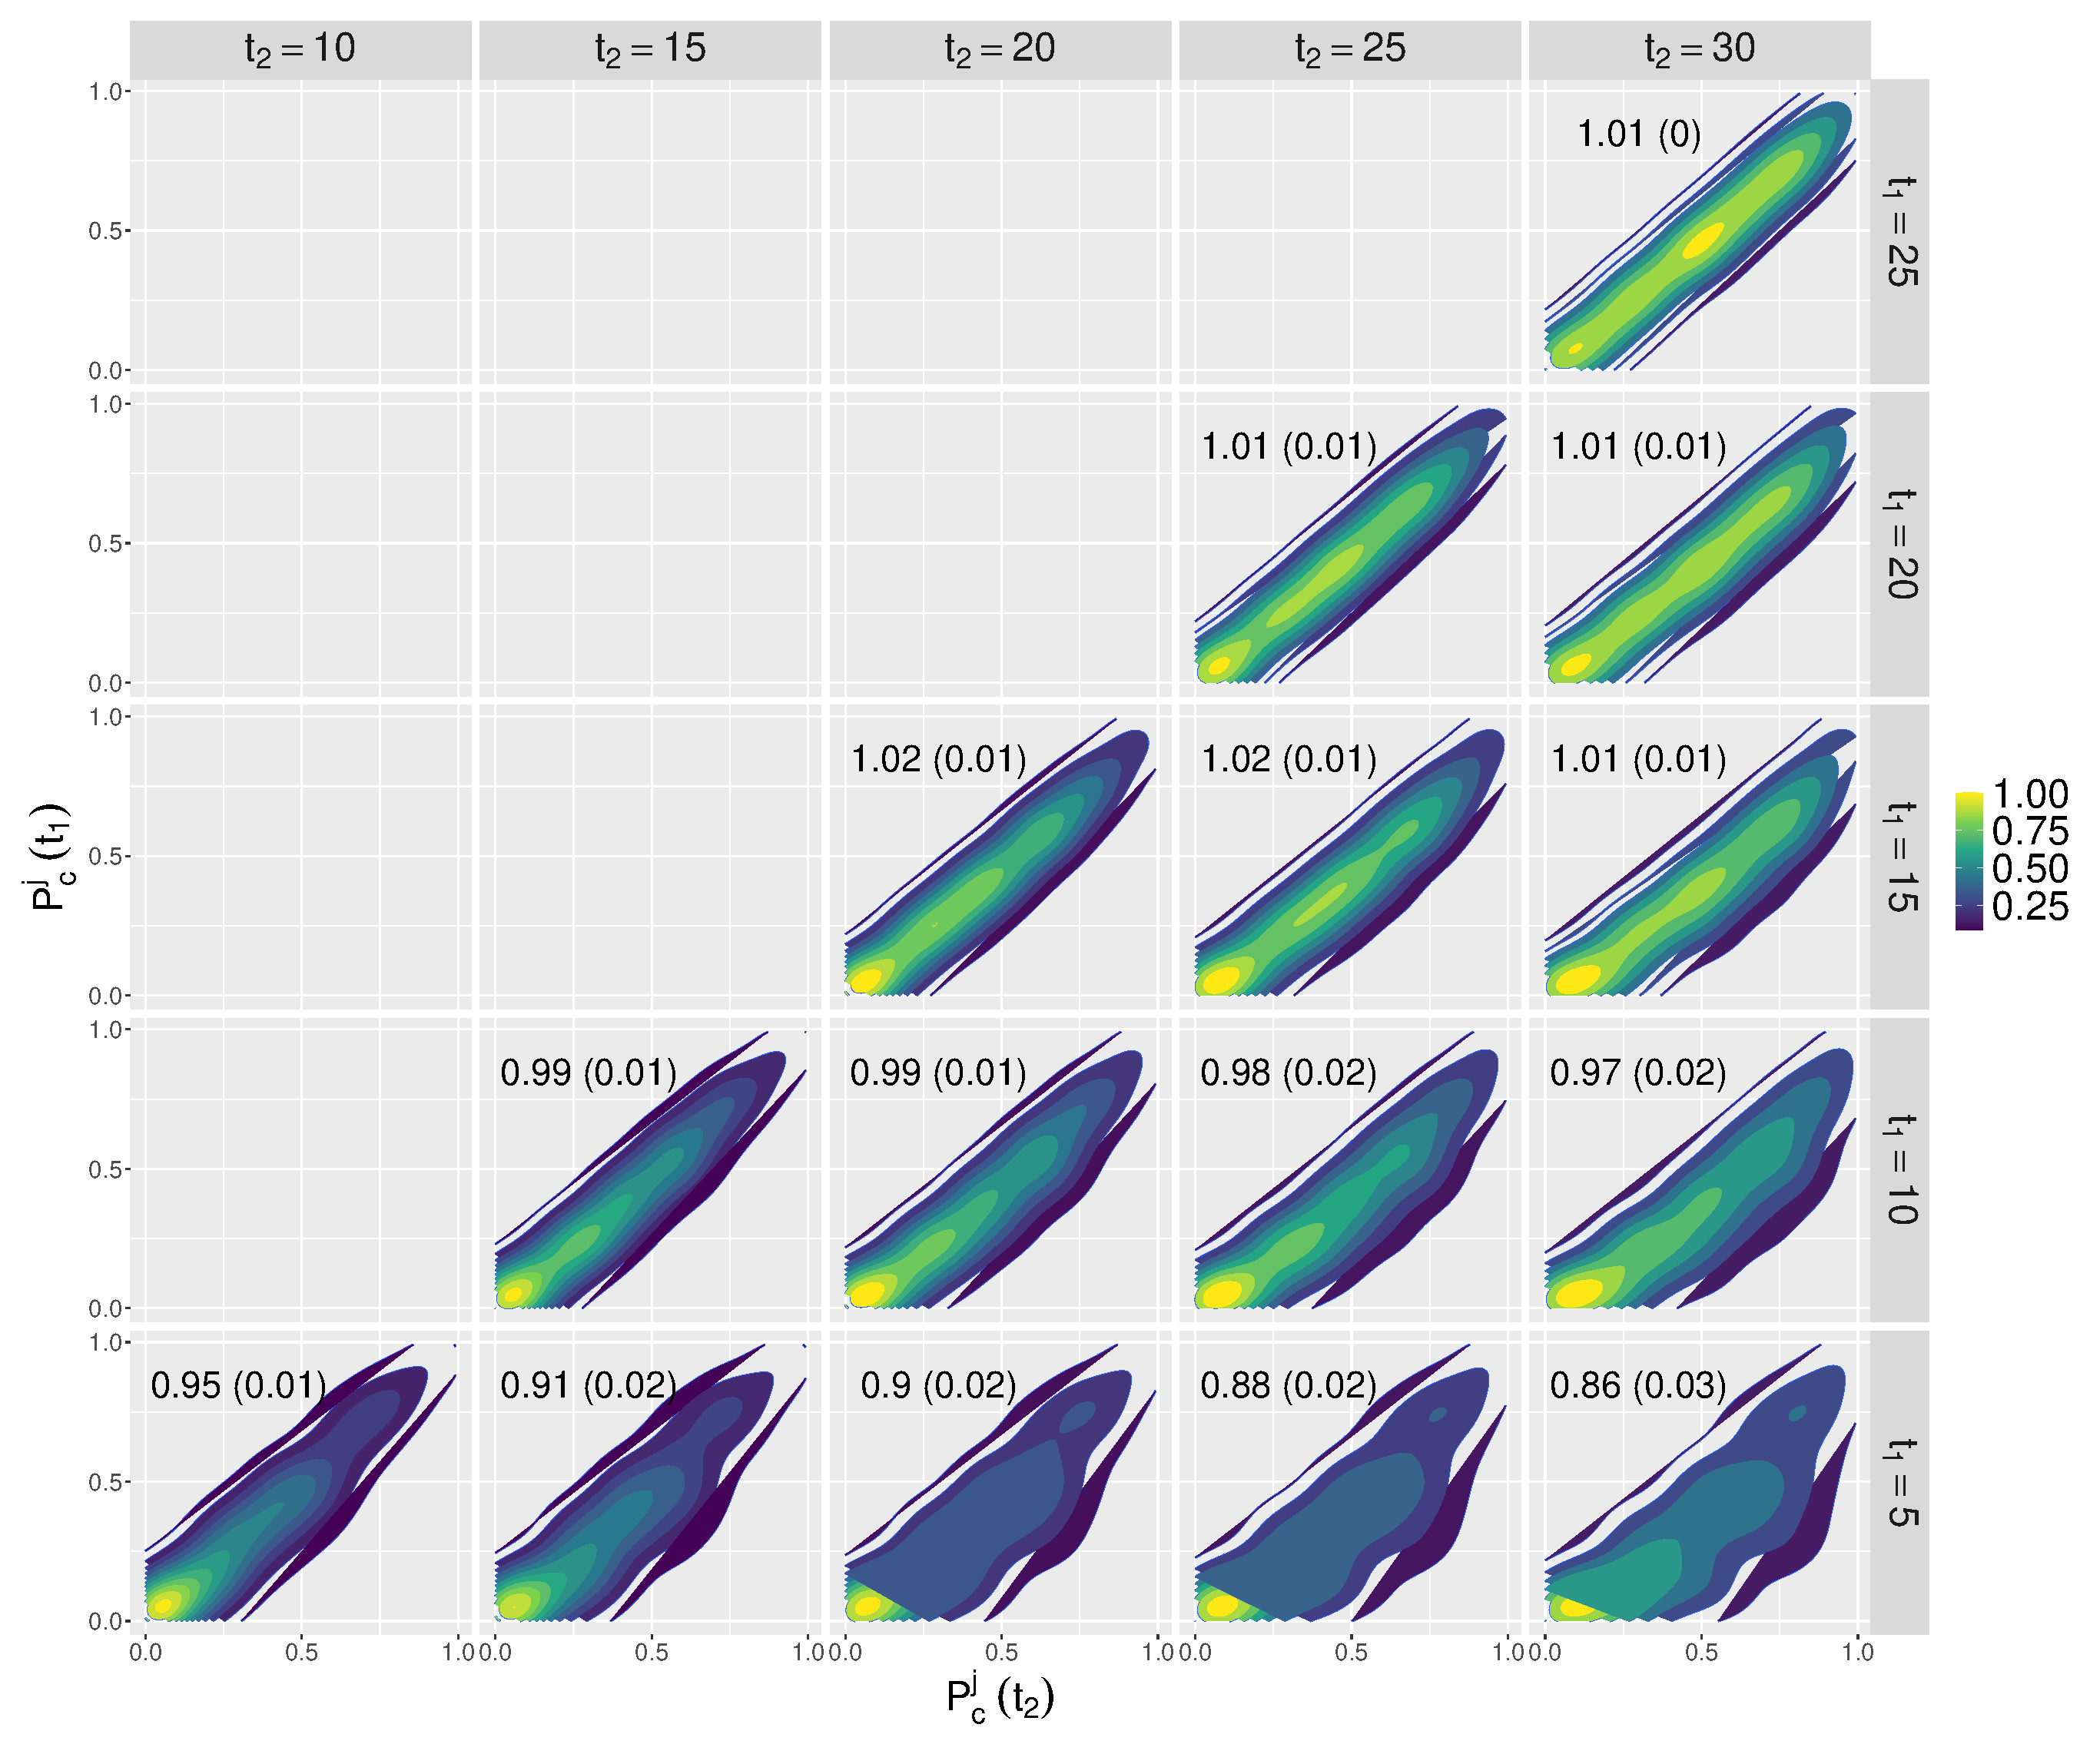
\includegraphics[width=\textwidth]{figures/pred_power/scatter_pubrp_bio1980.eps}
    \caption[Kernel density estimation for the scatter points of P$_c(t_1)$ and P$_c(t_2)$]{Kernel density estimation for the scatter points of P$_c^{jb}(t_1)$ and P$_c^{jb}(t_2)$. We also fitted a simple linear regression of P$_c^{jb}(t_2)$ on P$_c^{jb}(t_1)$. The estimated coefficient and the corresponding standard error (in parentheses) are displayed in each plot. The benchmark here includes publications in biology that were published in $1980$.}
    \label{fig:scatter_pubrp_bio1980}
\end{figure}


The strong linear relationship between P$_{c}^{jb}(t_1)$ and P$_c^{jb}(t_2)$ is further characterized in Figure \ref{fig:scatter_pubrp_bio1980}. The data are along the $45 \degree$ line, and the linear regression coefficient of P$_c^{jb}(t_2)$ on P$_c^{jb}(t_1)$ is close to $1$ with small standard errors, thus indicating the high stability of P$_c$. A similar figure for S$_{P5}$ is displayed in Supplemental Material Figure \ref{fig:scatter_autrp_all}, in which we find that S$_{P5}$ exhibits short-term stability.

Predicting S$_{P5}^{ib}(t_2)$ can assist in decision making for faculty positions or granting tenure, since the committee would like to examine the cumulative scientific impact of the scholar. In assigning research funding or allocating research resources regarding planned studies and potential future publications, the future impact of future works is often of interest. We utilize S$_{P5}^{ib}(t_2|t_1)$ to denote the rank percentile indicator calculated based on papers published between $t_1$ and $t_2$. Figure \ref{fig:hm_rp_aut_future} illustrates the correlation between S$_{P5}^{ib}(t_1)$ and S$_{P5}^{ib}(t_2|t_1)$. The magnitudes of correlation are moderately high, indicating an approximately linear relationship, although the strength is not as strong as it was in predicting the cumulative impact, that is, predicting S$_{P5}^{ib}(t_2)$, which is consistent with our expectation.

\subsection*{Predictive models}
We now formulate the prediction tasks as supervised learning problems, and we illustrate that the rank percentile indicators can be predicted via simple linear models. We consider the following fitting procedures; these models are ordered by increasing complexity:
\begin{itemize}
    \item Baseline: simple linear regression model.
    \item Simple Markov model (sm).
    \item Penalized linear regression models, including the ridge~\cite{hoerl1970ridge}, lasso~\cite{Tibshirani1996}, elastic net (enet)~\cite{zou2005regularization} and the Gamma lasso (gamlr)~\cite{Taddy2017}.
    \item Ensemble methods of regression trees, including the random forest (rf)~\cite{liaw2002classification} and extreme gradient boosting trees (xgbtree)~\cite{chen2016xgboost}.
    \item Neural networks (nnet).
\end{itemize}

The baseline model fits a simple linear regression of the target variable on the autoregressive feature, e.g. P$_c^{jb}(t_1)$ for predicting the publication impact. The simple Markov model further considers the change of the autoregressive feature in the past two ages, e.g. P$_c^{jb}(t_1)$-P$_c^{jb}(t_1-2)$, in addition to the autoregressive feature and fits a linear regression model. 

\subsubsection*{Features and model fitting}

For the rest of the methods, we created an extensive list of features based on the citation histories. The features are characterized as either scholar- or publication-based features. For example, to predict the scholar indicator S$_{P5}^{ib}(t_2)$, a scholar-based feature is the number of papers that scholar $i$ publishes by age $t_1$, and a publication-based feature is the average number of citations for these papers. We established a total of $30$ features for predicting the publication indicator and $42$ features for predicting the scholar indicator, which can be found in the Supplemental Material Tables \ref{tab:features_pubrp} and \ref{tab:features_autrp}, respectively. Note that many of the features have been utilized when formulating the prediction task for number of citations and h-index scores~\cite{acuna2012future,weihs2017learning}.

The features were created utilizing the citation information available by $t_1$, and the dependent variable was specified at $t_2$. The data was split into the training and testing set based on a 9:1 ratio. We considered five stages of a publication or a scholar, that is, $t_1\in\{5,10,15,20,25\}$, and we forecasted up to $30$ years of age, that is, $t_2=t_1+1,\cdots,30$; this resulted in $75$ pairs of $(t_1,t_2)$ in total. The models were independently trained $75$ times. 

We also noted (in the Supplemental Material Section \ref{sec:suppl_stationarity}) that both S$_{P5}$ and P$_c$ are non-stationary time series, as evidenced by the Dicky-Fuller test~\cite{dickey1979distribution} and the KPSS test~\cite{kwiatkowski1992testing}. The differenced series are stationary (also presented in the Supplemental Material) and are utilized as the response variable, that is $\Delta \text{P}_{c}^{jb}(t_2) = \text{P}_{c}^{jb}(t_2) - \text{P}_{c}^{jb}(t_1)$, $\Delta \text{S}_{P5}^{ib}(t_2) = \text{S}_{P5}^{ib}(t_2) - \text{S}_{P5}^{ib}(t_1)$, and $\Delta \text{S}_{P5}^{ib}(t_2|t_1) = \text{S}_{P5}^{ib}(t_2|t_1) - \text{S}_{P5}^{ib}(t_1)$. Note that the stationarity discussed here characterizes the property of S$_{P5}$ and P$_c$ as time series. It is different from the stationarity as discussed in Figure \ref{fig:rp_stationarity}, where we fix $t=10$ and examine the stationarity of S$_{P5}(10)$ over the starting year of the scholars' careers.

The machine learning methods were trained using \textit{R}~\cite{RCT2019} with the package \textit{mlr}~\cite{Bischl2016}, which provides a pipeline of training, validating, and testing for the model. The lasso, ridge, elastic net, random forest, and xgbtree are inbuilt learners of the package. The Gamma lasso and neural network were trained utilizing \textit{R} packages \textit{gamlr}~\cite{Taddy2017} and \textit{keras}~\cite{Allaire2019}, respectively. 

The machine learning methods require hyperparameter tuning, which involves deciding the search space of parameters and evaluating the sets of parameters utilizing the validation data. The optimal model is the one that minimizes the validation error. The hyperparameters for each machine learning model considered in this paper are presented in Supplemental Material Table \ref{tab:hyperpara}. The parameter space can be substantial for methods such as xgbtree, which utilizes an extensive list of tunable parameters. We applied Bayesian optimization, which searches over the parameter space based on the performance gain.


\subsubsection*{Results}

The prediction accuracy is presented in Figure \ref{fig:pred_r2}. We see 
that the baseline model predicts the cumulative impacts, P$_c^{jb}(t_2)$ and S$_{P5}^{ib}(t_2)$, well, and the usage of a large number of features and complex machine learning models offers little improvement. Predicting the future impact of scholars, S$_{P5}^{ib}(t_2|t_1)$, is more difficult. The baseline model can still provide reasonable predictions, but the performance is not as satisfactory as others, especially when $t_1$ is large. By simply adding the difference $\text{S}_{P5}^{ib}(t_1) - \text{S}_{P5}^{ib}(t_1-2)$ as an extra feature, the simple Markov model achieves similar performance compared to the complex machine learning models, which rely on an extensive list of features and exhibit non-linear relationships. Other types of evaluation metrics for the predictive models, including the root mean squared error, root median squared error, and mean absolute error, can be found in the Supplemental Material (Figures \ref{fig:pred_rmse}, \ref{fig:pred_medse}, and \ref{fig:pred_mae}, respectively). 

\begin{figure}[ht!]
    \centering
    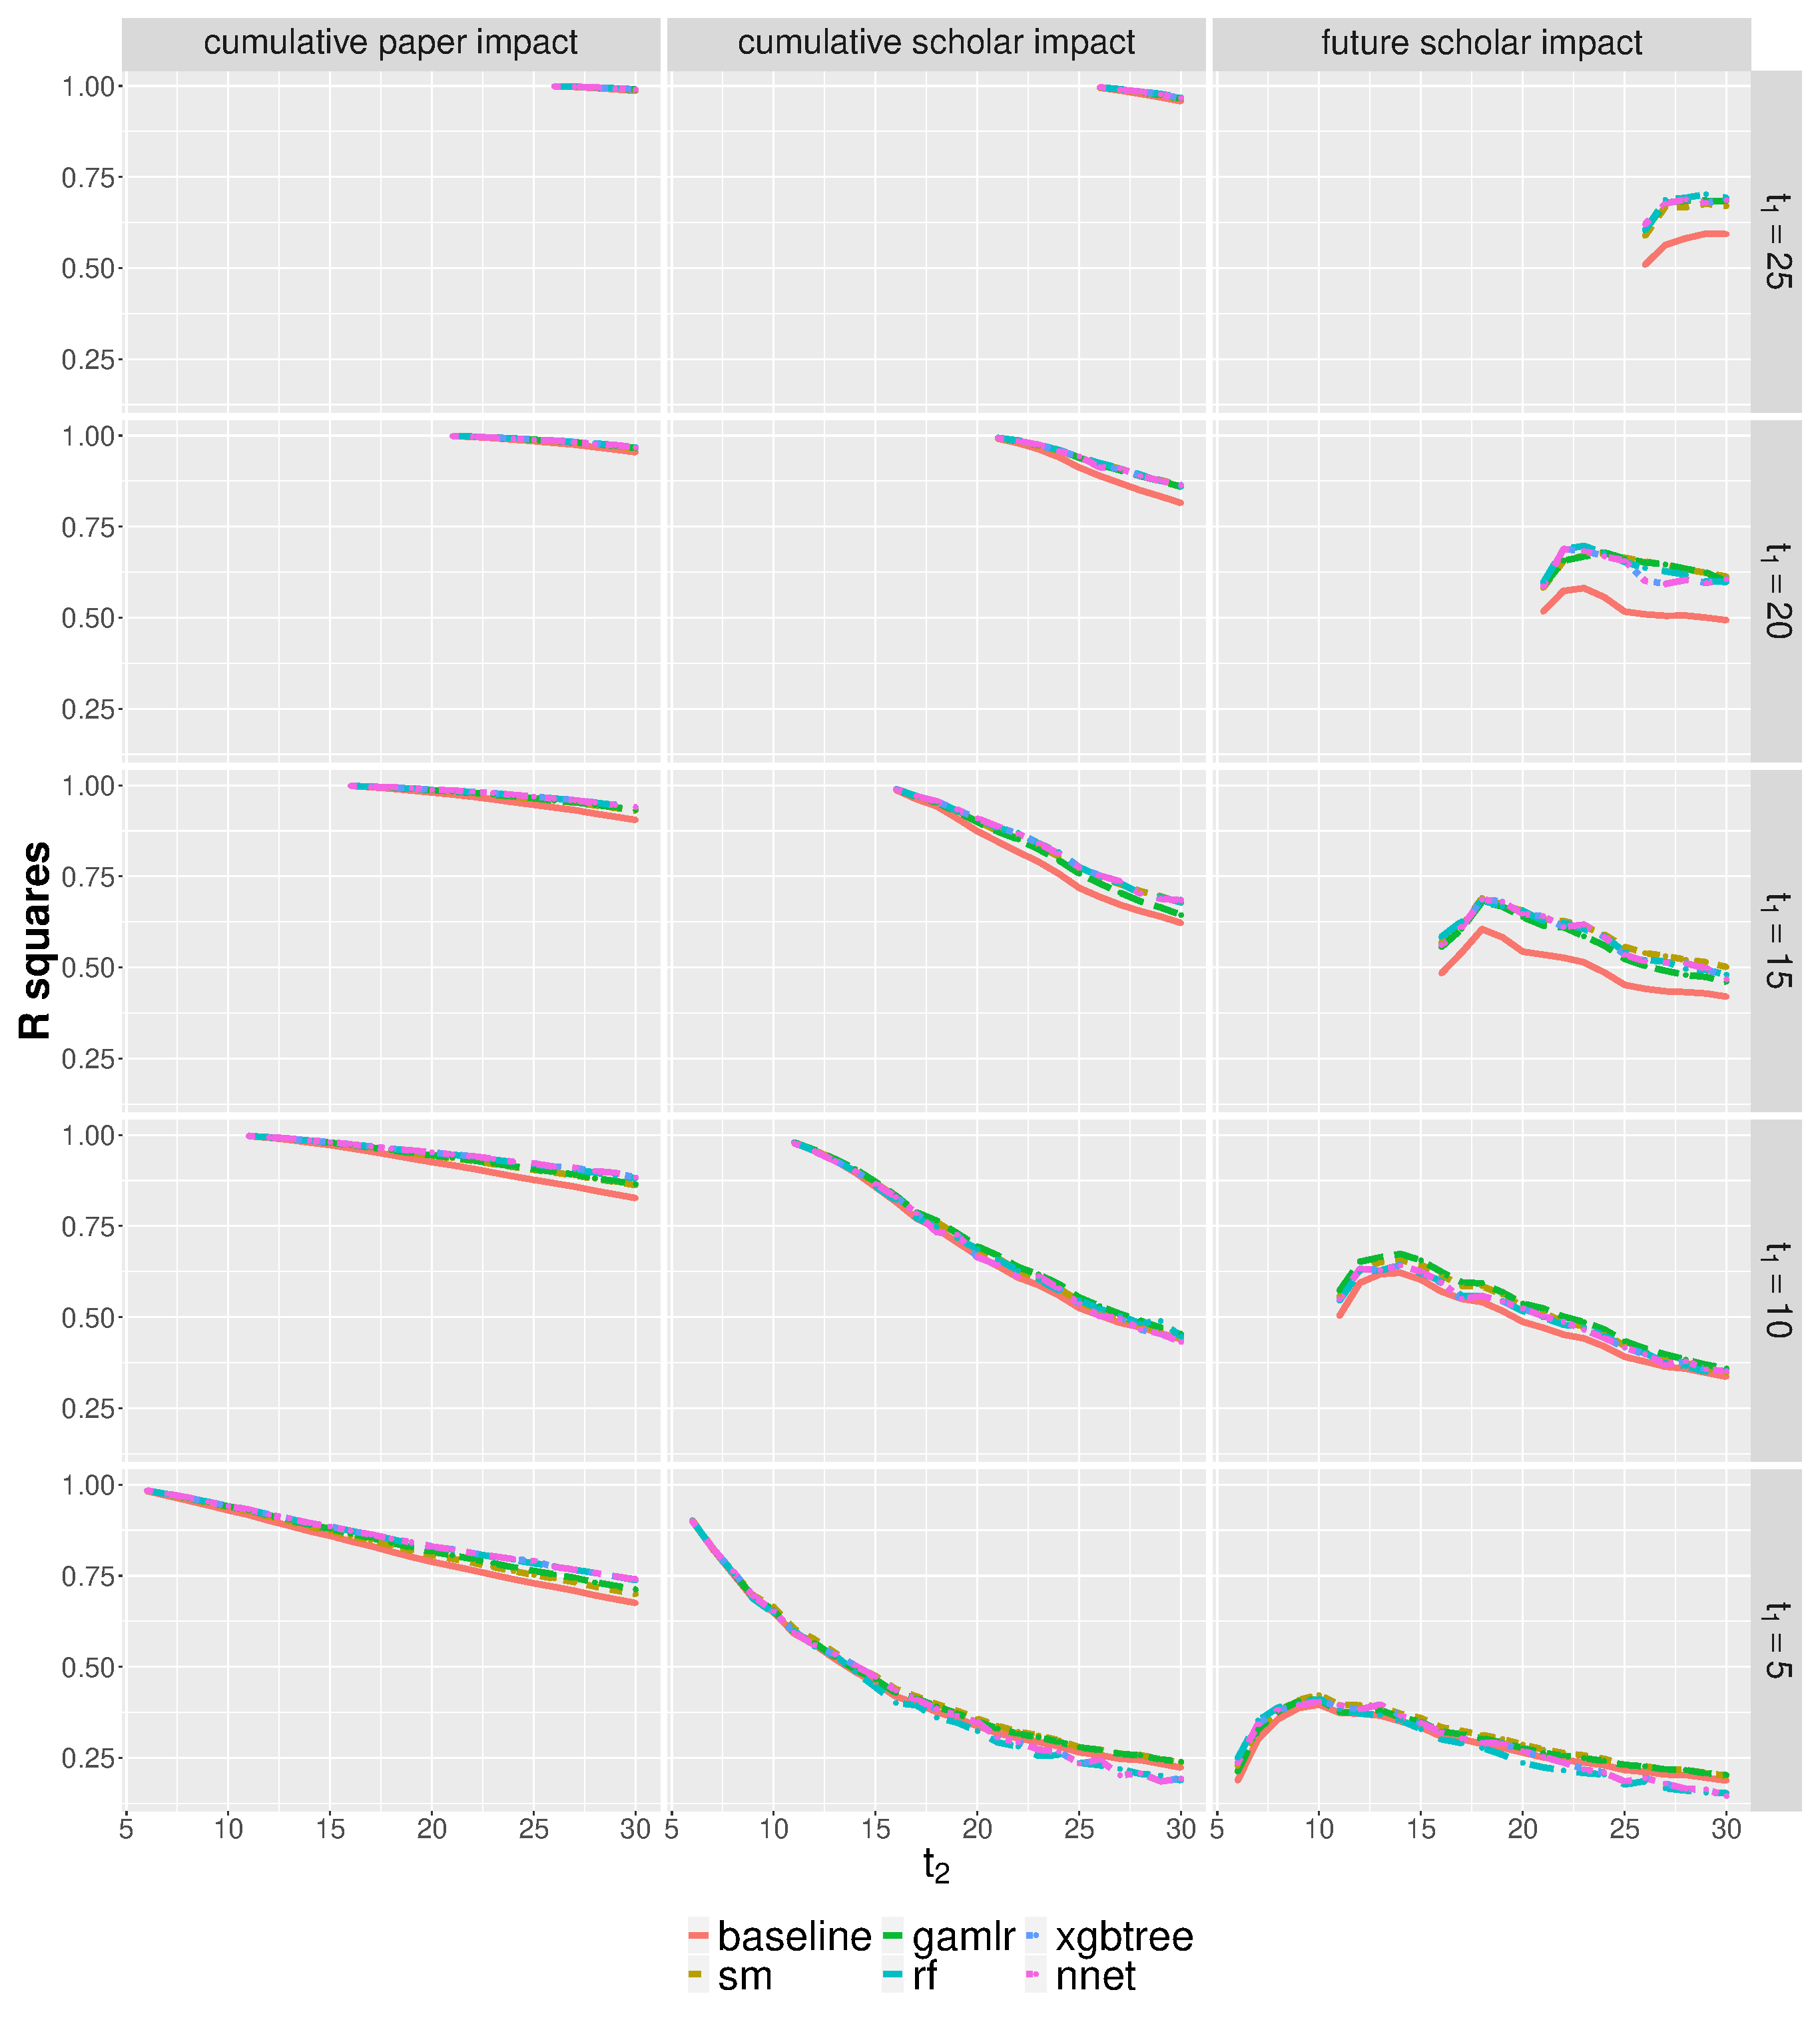
\includegraphics[width=\textwidth]{figures/pred_model/r2.eps}
    \caption[R squares of the predictive models]{Testing $R^2$ of the predictive models. The lasso, ridge, and elastic net are outperformed by the Gamma lasso and hence are ignored for a better visualization.}
    \label{fig:pred_r2}
\end{figure}






